\documentclass[review]{elsarticle}


\usepackage{mathtools}
\usepackage{lineno,hyperref}
\modulolinenumbers[5]
\usepackage{subfigure}
\journal{Journal of \LaTeX\ Templates}

%%%%%%%%%%%%%%%%%%%%%%%
%% Elsevier bibliography styles
%%%%%%%%%%%%%%%%%%%%%%%
%% To change the style, put a % in front of the second line of the current style and
%% remove the % from the second line of the style you would like to use.
%%%%%%%%%%%%%%%%%%%%%%%

%% Numbered
%\bibliographystyle{model1-num-names}

%% Numbered without titles
%\bibliographystyle{model1a-num-names}

%% Harvard
%\bibliographystyle{model2-names.bst}\biboptions{authoryear}

%% Vancouver numbered
%\usepackage{numcompress}\bibliographystyle{model3-num-names}

%% Vancouver name/year
%\usepackage{numcompress}\bibliographystyle{model4-names}\biboptions{authoryear}

%% APA style
%\bibliographystyle{model5-names}\biboptions{authoryear}

%% AMA style
%\usepackage{numcompress}\bibliographystyle{model6-num-names}

%% `Elsevier LaTeX' style
\bibliographystyle{elsarticle-num}
%%%%%%%%%%%%%%%%%%%%%%%

\begin{document}

\begin{frontmatter}

\title{Combining thermo-elastic $r$-adaptation and sensor-based $p$-adaptation for compressible flows}
\tnotetext[mytitlenote]{Fully documented templates are available in the elsarticle package on \href{http://www.ctan.org/tex-archive/macros/latex/contrib/elsarticle}{CTAN}.}

%% Group authors per affiliation:
\author{D. Ekelschot, D. Moxey, S.J. Sherwin and J. Peir\'{o}}
\address{Imperial College London, South Kensington Campus, London}
\fntext[myfootnote]{}

%% or include affiliations in footnotes:
%\author[mymainaddress,mysecondaryaddress]{Elsevier Inc}
%\ead[url]{www.elsevier.com}

%\author[mysecondaryaddress]{Global Customer Service\corref{mycorrespondingauthor}}
\cortext[mycorrespondingauthor]{Dirk Ekelschot}
\ead{de912@ic.ac.uk}

%\address[mymainaddress]{Imperial College London, South Kensington Campus, London}
%\address[mysecondaryaddress]{360 Park Avenue South, New York}

\begin{abstract}
 In this article, we present a $r$-adaptation (adaptation through redistribution) capability to improve compressible flow solutions that exhibit shock waves. 	The proposed $r$-adaptation strategy uses a mesh deformation capability that relies on a thermo-elastic analogy which was originally intended to control mesh validity in the framework of the high-order spectral/$hp$ element approach \cite{Moxey2015}.  
 In this work, the position of the shock wave is detected using a discontinuity sensor \cite{Persson2006}.
We present the idea of extending the use of this discontinuity sensor as a thermal stress term in the thermo-elastic formulation to {\it cool down}, and therefore contract, the elements that are in the vicinity of shock waves. Thereby, we improve the representation of the shock wave while maintaining the same number of degrees of freedom. Furthermore, this $r$-adaptation capability is combined with a sensor-based $p$-adaptation strategy which we apply to improve the accuracy of the smooth parts of the solution.
\end{abstract}
\begin{keyword}
Compressible flows, high-order spectral/$hp$ discontinuous Galerkin, $r$-adaptation, sensor-based $p$-adaptation
\end{keyword}

\end{frontmatter}

\linenumbers


\section{Introduction}

\par The aeronautical industry uses computational fluid dynamics (CFD) technologies to obtain a better understanding of complex physical phenomena that occur when compressible flow passes a geometry like an aircraft for example.		The compressible fluid equations are non-linear and flow disturbances move along characteristic lines with a speed that depends on the solution itself.	This results in flow features like shock waves and contact discontinuities which are anisotropic by nature and occur in concentrated regions of the computational domain.		
Generally, it is the desire to predict the location and strength of shock waves accurately in order to obtain an accurate estimate of the wave drag for example.	
Furthermore, under-resolving shock waves leads to the generation of numerical oscillations (Gibbs phenomena) which may result eventually in the divergence of the solution itself.


\par Anisotropic mesh adaptation capabilities are used to improve the accuracy of the solution in the vicinity of shock waves while keeping the computational cost to a minimum.	 In the framework of a high-order spectral/$hp$ element discretisation, we can generally achieve an improvement in accuracy by reducing the element size ($h$) or increasing the approximation order ($p$).	 However it is preferred to decrease the element size and use a low approximation order~\cite{Ekelschot2016} to approximate shock waves so that further numerical oscillations are avoided.		


\par The generation of these anisotropic (adapted) meshes to improve the flow solution near the shock wave is not straightforward and this received a significant amount of attention in the literature.		 Initially,  Peraire et al. \cite{Peraire1987,Peraire1992} proposed a complete re-meshing of the computational domain based on directional properties of the interpolation error.	Mavripilis \cite{mavriplis1990} proposed to generate anisotropic elements based on a Delaunay approach in two dimensions to obtain anisotropic mesh in the wake and boundary layer regions.		George et al. \cite{George1991}  showed that the absolute value of the Hessian of the solution is a metric and can serve as a Riemannian metric space which can be used to generate anisotropic mesh.		A mesh is obtained for which the direction and stretching (anisotropy) of the local mesh is aligned with the anisotropy of the solution by first generating a unit mesh in this defined Riemannian metric space and projecting it back onto the original Euclidean metric space.		More recently, this idea has been adopted to perform anisotropic mesh adaptation where the aim is to minimize the interpolation error based on the Hessian of the solution and the local metric of the mesh \cite{Alauzet2016,Loseille2009b,Loseille2011a,Loseille2011b}.
Most of the adaptation strategies proposed in the aforementioned papers rely on element splitting or adding additional degrees of freedom locally ($h$-refinement) to improve the accuracy.


\par The aim of this article is to present a proof-of-concept $rp$-adaptation strategy (adaptation through redistribution) to optimally redistribute the degrees of freedom so that the solution accuracy near shock waves is improved while keeping the number of degrees of freedom constant.
	 We use the high-order spectral/$hp$ element code Nektar++ \cite{Cantwell2015} and we are exploiting the available mesh deformation capability that relies on a thermo-elastic analogy which is originally intended to control mesh validity \cite{Moxey2015}.		The mesh is treated as an elastic solid and thermal stresses are incorporated in the elastic formulation to locally {\it cool down} (contract) or {\it heat up} (expand) elements depending on where mesh refinement is required.		The shock position is detected using the discontinuity sensor introduced by Persson and Peraire \cite{Persson2006} and the thermal-stresses that drive the $r$-adaptation are derived from this discontinuity sensor.	
	

\par This sensor is also exploited as a local error indicator since it quantifies the local smoothness of the solution within each element. The approximation order ($p$) can be increased or decreased based on the value of the discontinuity sensor and a set of threshold values. Hence, additionally, we combine the proposed $r$-adaptation strategy with a sensor-based $p$-adaptation capability.


\par This article is structured as follows: Firstly, the governing equations are introduced both in the continuous and discrete form. Secondly, the $r$-adaptation capability that uses a thermo-elastic analogy is introduced.	 	Thirdly, the brief overview of the used sensor-based $p$-adaptation algorithm is given.	This is followed by a discussion of the implementation of both the $r$- and $p$-adaptation capabilities.	The demonstration of the combination of $r$-adaption with sensor-based $p$-adaptation is shown in the fifth section for two test cases.	Firstly, $rp$-adaptation is illustrated using a supersonic flow past a forward facing step and secondly, the $rp$-adaptation strategy is applied to transonic flow $(M=0.8)$ past a NACA $0012$ at an angle of attack of $1.25^\circ$.	We finish with conclusions and recommendations that are based on the numerical results presented in this article.
    

\section{The governing equations}
In this section, we discuss the continuous form of the governing equations. 
We consider steady compressible flows in a domain, $\Omega$, and we assume that the effects of viscosity and heat conduction are neglected.  The steady compressible Euler equations are given by
\begin{equation}
{\bf R}({\bf u}) = \sum_{i=1}^2\frac{\partial }{\partial x_i}{\bf f}_i^c({\bf u}) = {\bf 0}; \qquad {{\bf u}}\in \Omega\label{eq:EU}
\end{equation}
The two-dimensional Cartesian frame of reference has coordinates $(x_1,x_2)$. The vector of conserved variables 
is given by  \mbox{${\bf u} = \{ u_1, u_2, u_3, u_4 \}^t = \{\rho, \rho v_1, \rho v_2, \rho E\}^t$} where 
$\rho$ is the density, $v_1$ and $v_2$ are the Cartesian components of the velocity, and $E$ is the total energy.
$\bf R({\bf u})$ denotes the differential operator representing the governing equations. The two-dimensional Cartesian components of the convective fluxes, ${{\bf f}}^c_1$ and ${{\bf f}}^c_2$, are given by
\begin{equation}\label{eq:convflux}
%\begin{split}
{{\bf f}}_1^c=\left\{ {\begin{array}{c}
\rho v_1\\
P+\rho v_1^2 \\
\rho v_1 v_2 \\
\rho v_1 H\\
\end{array} } \right\},\quad 
{{\bf f}}_2^c=\left\{ {\begin{array}{c}
\rho v_2\\
\rho v_1v_2 \\
P + \rho v_2^2  \\
\rho v_2 H\\
\end{array} } \right\}
%\end{split}	
\end{equation}
where $H$ is the total enthalpy and $P$ is the pressure. The total enthalpy is defined as
\begin{equation}
H = E + \frac{P}{\rho}
\end{equation}
To close the system, the pressure for a perfect gas is given by
\begin{equation}
P  = (1 - \gamma) \rho \left(E-\frac{v_1^2+v_2^2}{2}\right)
\end{equation}
where $\gamma = \frac{c_v}{c_P}$ is the ratio of specific heats and its value for air is $\gamma = 1.4$. 
\subsection{Boundary conditions}
As mentioned in the previous sections, the governing equations are solved in a bounded domain. We consider the compressible Euler equations and, as a result, we model a solid wall of the body by considering that the normal component of the velocity is equal to zero. Hence, the solid wall boundary condition is written as
\begin{equation}\label{eq:bcwall}
\sum_{i=1}^2v_i n_i=0; \qquad {{\bf u}}\in \Gamma_w
\end{equation}
where $\Gamma_w$ denotes the wall boundary.
\par Generally, we consider a finite computational domain and we require a far-field boundary condition which dictate the solution is equal to the free-stream flow conditions. We therefore write
\begin{equation}\label{eq:bcff}
\bf u=\bf u_\infty; \qquad {{\bf u}}\in \Gamma_\infty
\end{equation}
\section{The high-order spectral/$hp$ discontinuous Galerkin discretisation} 
In this section, we describe the high-order spectral/$hp$ discretisation that is used to calculate the discrete solution to the governing equations that were introduced in the previous section. 
We start off by introducing an additional artificial diffusion term that is required to enable the calculation of compressible inviscid solutions with shock waves. We consider the shock capturing technique proposed by Persson and Peraire \cite{Persson2006}. Equation (\ref{eq:EU}) becomes
\begin{equation}\label{eq:EUdiff}
{\bf R}({\bf u}) = \sum_{i=1}^2\frac{\partial }{\partial x_i}{\bf f}_i^c({\bf u})-\mu_a\frac{\partial^2 {\bf u}}{\partial x_i^2}={\bf 0}; \qquad {{\bf u}}\in \Omega
\end{equation}
where $\mu_a$ is an artificial viscosity coefficient that depends on a shock sensor which we will discuss once a weak discrete form of equation (\ref{eq:EUdiff}) is derived.
\par We adopt a similar mixed formulation as the one that is presented by Bassi and Rebay \cite{Bassi1996} to deal with the second order derivative terms in equation (\ref{eq:EUdiff}). Hence, we write equation (\ref{eq:EUdiff}) as
\begin{eqnarray}\label{eq:EUmixed}
{\bf g} - \nabla {\bf u}&= \bf {\bf 0}\label{eq:EUmix1}\\
\sum_{i=1}^{2}\frac{\partial }{\partial x_i}\left({\bf f}^c_i({\bf u})-\mu_a(s_e){\bf g}_i\right) &= {\bf 0}\label{eq:EUmix2}
\end{eqnarray}
We first solve for the first order derivatives of $\bf u$ using equation \ref{eq:EUmix1} which we then substitute in the discrete form of equation (\ref{eq:EUmix2}).
\par This mixed formulation is discretised using the high-order spectral/{$hp$} discontinuous Galerkin method available in Nektar++ \cite{Cantwell2015}. 
The computational domain, $\Omega$, is subdivided into $N_{el}$ non-overlapping elements, so that
$\Omega = \bigcup_{e=1}^{N_{el}}\Omega_e$, where $\bigcap_{e=1}^{N_{el}}\Omega_e=\emptyset$.  
By using an appropriate mapping $M_e:(x_1,x_2)\mapsto(\xi_1,\xi_2)$, we map the local element coordinates $(x_1, x_2)$ to reference element coordinates $(\xi_1,\xi_2)$ for which hold that $-1\leq \xi_1,\xi_2\leq 1$. All mathematical operations take place in this reference space which is one of the fundamental aspects of the finite element method (FEM).
\par Initially, the weak form of the first equation (\ref{eq:EUmix1}) is obtained using the method of weighted residuals which dictates that the governing equations are multiplied with a test function, $v$. This product is then integrated over the domain and the result is set equal to zero. 
\begin{equation}\label{eq:eq1coup}
\int_{\Omega}{v} \left({\bf g}-\nabla{\bf u}\right) d\Omega= \bf 0
\end{equation}
Using Gauss' theorem and using the fact that the domain is subdivided into $N_{el}$ non-overlapping elements, equation (\ref{eq:eq1coup}) becomes
\begin{equation}\label{eq:eq1coupled}
\sum_{e=1}^{N_{el}}\int_{\Omega_e}{v^\delta_e} {{{\bf g}}}^\delta_e \, d\Omega-\int_{\Gamma_e}{v^\delta_e}{\bf u}^\delta_e  \vec{n}\, d\Gamma + \int_{\Omega} \nabla {v}^\delta_e {\bf u}^\delta_e \, d\Omega= \bf 0
\end{equation}
In contrast to the classical FEM, we approximate the solution within each element, ${\bf u}_e$, using a summation of polynomial expansion functions which are weighted using a set of coefficients that ultimately are the degrees of freedom that we are solving for. Furthermore, we utilise a discontinuous Galerkin discretisation for the governing equations meaning that we define that the solution and test functions are both discontinuous at the interface between elements. 
Hence, the local solution can be expressed as ${{\bf u}}^\delta_e$ and therefore we write,
\begin{equation}\label{eq:sol}
{{\bf u}}^\delta_e(M_e(x_1,x_2))=\sum_{p=0}^{P}\sum_{q=0}^{Q}\phi_{pq}({\xi_1},{\xi_2})\bar{u}_{pq}
\end{equation}
where the array $\bar{u}_{pq}$ denotes the degrees of freedom that we solve for and $\psi_{pq}$ represents the two-dimensional expansion functions. In this case we use the modified basis \cite{BookSpencer}.
The Galerkin discretisation dictates that the test function uses the same polynomial expansion functions as the solution and therefore we write
\begin{equation}\label{eq:test}
v_e^\delta(M_e(x_1,x_2)) = \phi_{pq}({\xi_1},{\xi_2})
\end{equation}

Substituting equations (\ref{eq:sol})-(\ref{eq:test}) into equation (\ref{eq:eq1coupled}), we obtain the discrete weak form of the governing equations
\begin{equation}\label{eq:eq1coupleddisc}
\sum_{e=1}^{N_{el}}\left\{\int_{\Omega_e}{v}_e {{{\bf g}}}^\delta_e \, d\Omega-\int_{\Gamma_e}{v}^\delta_e{\bf u}^\delta_e  \vec{n}\, d\Gamma + \int_{\Omega_e} \nabla {v}_e {\bf u}^\delta_e \, d\Omega\right\}= \bf 0
\end{equation}
We calculate a solution for the first order derivatives $\bf g_e^\delta$ and they are substituted into equation (\ref{eq:EUmix2}). The weak form of (\ref{eq:EUmix2}) is obtained using the same approach that is used to derive (\ref{eq:eq1coupleddisc}). We write
\begin{eqnarray}\label{eq:discEuler}
&\sum_{e=1}^{N_{el}}\ \left\{- \int_{\Omega_e}\sum_{i=1}^{2} \frac{\partial v_e^\delta}{\partial x_i} \left({\bf f}^c_i({\bf u}^\delta_e)-\mu_a(s_e){\bf g}_{i,e}^\delta\right)\ d{\Omega}\right\}\\ \nonumber
+&\sum_{e=1}^{N_{el}}\ \left\{ \int_{\Gamma_e} v_e^\delta\sum_{i=1}^2\left( {\bf f}^c_i({\bf u}^\delta_e)-\mu_a(s_e){\bf g}_{i,e}^\delta\right)n_i\ d\Gamma\right\}  = 0
\end{eqnarray}
The solution at each interface between the elements is represented twice due to the discontinuous nature of DG. The integrand in the boundary integral of equation (\ref{eq:discEuler}) is substituted by a numerical flux function. We calculate the numerical flux through each interface using a Riemann solver.
\begin{equation}\label{eq:RiemannGov}
\left .\sum_{i=1}^2{\bf f}^c_i({\bf u_e^\delta}) n_i\right |_{\Gamma_e} \approx \mathcal{H}^c({{\bf u}^\delta_{e,ex}},{{\bf u}^\delta_{e,in}};\vec{n})
\end{equation}
where ${\bf u}^\delta_{e,ex}$ and ${\bf u}^\delta_{e,in}$ are the conservative variables on the external and internal interface with respect to the $e^{th}$ element. This mechanism allows information to pass from one element to the other.
The boundary terms in equations (\ref{eq:eq1coupleddisc}) and (\ref{eq:discEuler}) that follow from the discretisation of the diffusive term are also substituted by numerical flux functions. In this case, we use the local discontinuous Galerkin (LDG) formulation \cite{CockburnShu1997}.
Therefore we use the external state variables in equation (\ref{eq:eq1coupleddisc}) to calculate the flux at the boundary and 
write
\begin{eqnarray}\label{eq:viscflux1}
\left . {\bf u}^\delta_e \vec{n} \right |_{\Gamma_e} = {\bf u}^\delta_{ex}\vec{n}
\end{eqnarray}
Further, we replace  the term $\sum_{i=1}^2{\bf g}_{i,e}^\delta n_i$ in the boundary integral in equation (\ref{eq:discEuler}) with the internal first order derivatives as
\begin{eqnarray}\label{eq:viscflux2}
\left .{\sum_{i=1}^2{\bf g}_{i,e}^\delta n_i}\right |_{\Gamma_e} = \left .{\sum_{i=1}^2{\bf g}_{i,in}^\delta n_i}\right |_{\Gamma_e}
\end{eqnarray}
\subsection{The discrete form of the boundary conditions}
The boundary conditions presented in equations (\ref{eq:bcwall}) and (\ref{eq:bcff}) are imposed weakly through the solution of a Riemann problem.
At the boundary, we consider a ghost state that resembles ${\bf u}_{ex}$ in the previous analysis. 
By considering the inner state of the solution and the propagation of information dictated by the characteristic analysis (Riemann solver), we can appropriately impose the correct state solution at this ghost state.
\begin{equation}\label{eq:ghost_slip_1}
\vec{v}_{ex} = \vec{v}_{in}-2\left(\vec{v}_{in}\cdot\vec{n}\right)\vec{n}; \qquad {{\bf u}}\in \Gamma_w
\end{equation}
At the far-field boundary, we calculate the boundary values again through the solution of a Riemann problem. In this case, depending on the sign of the velocity vector, we are dealing with an inflow or outflow conditions. Considering subsonic outflow for example, we state that the Riemann invariants corresponding to the positive characteristics are determined by the internal values and the Riemann invariant corresponding to the negative characteristics are determined by the far-field conditions. Based on these Riemann invariants, we calculate the appropriate values of the solution at the far-field considering the characteristic analysis and the sign of the normal velocity with respect to the far-field boundary \cite{ToroRiemann}.
\par For supersonic inflow this analysis is significantly simplified because we know that all Riemann invariants are determined by the external state and we can write
\begin{equation}
{\bf u} = {\bf u}_{ex};\qquad {{\bf u}}\in \Gamma_\infty
\end{equation}
while for supersonic outflow holds that the Riemann invariants are completely defined by the internal state and we can write
\begin{equation}
{\bf u} = {\bf u}_{in};\qquad {{\bf u}}\in \Gamma_\infty
\end{equation}
\subsection{Shock capturing technique}
To finalise the section on the discretisation of the governing equations, we describe the formulation of the discontinuity sensor and the artificial viscosity coefficient. The discontinuity sensor detects the shocks by quantifying the smoothness of the solution within an element. It does this by comparing the solution within an element at the given approximation order $p$ and a reduced order $p-1$ \cite{Persson2006}. Hence, the discontinuity sensor is given by
\begin{equation}\label{eq:sensor}
s_e=\log_{10}\left(\frac{||f({\bf u}^p_e)-f({\bf u}^{p-1}_e)||_{L_2}}{||f({\bf u}_e^p)||_{L_2}}\right)
\end{equation}
where $f({\bf u}^p_e)$ represents a general function within the $e^{th}$ element that depends on the conservative variables at order $p$. The sensor can be based on the conservative variables directly or based on the Mach number or pressure for example.
Artificial viscosity is added to the elements that are highlighted by $s_e$. The value of $\mu_a$ is determined by
\begin{eqnarray}\label{eq:mua}  \mu_a(s_e)
=\left \{ \begin{array}{l}
      0\hspace{46mm}\mbox{if}\hspace{10mm}s_e<s_0-\kappa\\  
     \frac{\mu_{max}}{2}\left(1+\sin{\left(\frac{\pi\left(s_e-s_0\right)}{2\kappa}\right)}\right)\hspace{6mm}\mbox{if}\hspace{10mm}s_0-\kappa<s_e<s_0+\kappa\\
     \mu_{max}\hspace{42mm}\mbox{if}\hspace{10mm}S_e>s_0+\kappa
    \end{array} 
    \right.
\end{eqnarray}
where $\kappa$ and $s_0$ are quantities that define the range of sensor values that require artificial viscosity. The value of $\mu_{max}$ defines the maximum amount of artificial viscosity that is added. These values are determined empirically \cite{Persson2006}.
\section{$r$-adaptation using a thermo-elastic analogy}
The aim of this section is to introduce the $r$-adaptation capability that uses a thermo-elastic analogy. Initially, the mesh deformation strategy that uses this formulation was developed to control mesh validity in the framework of the high-order spectral/$hp$ element approach where the thermo-elastic equations were used to deform a straight sided high-order elements to accommodate for curved boundaries \cite{Moxey2015}.

\par We exploit the available thermo-elastic analogy to perform $r$-adaptation (adaptation trough redistribution). We incorporate the concept of thermal expansion and contraction that is known from the theory of solid mechanics. The elements that are highlighted by the discontinuity sensor, which is defined in equation (\ref{eq:sensor}), are {\it cooled down} and in this way reduced in size. We want to determine a vector field, ${\bf q}$, that dictates the displacements of the nodes using the thermo-elastic analogy and that specifically targets shock waves. A sketch is given in figure \ref{fig:sketch}.
\begin{figure}[!htbp]
\begin{center}
%\includegraphics[width=0.6\textwidth]{figures/defomation_sketch2.pdf}
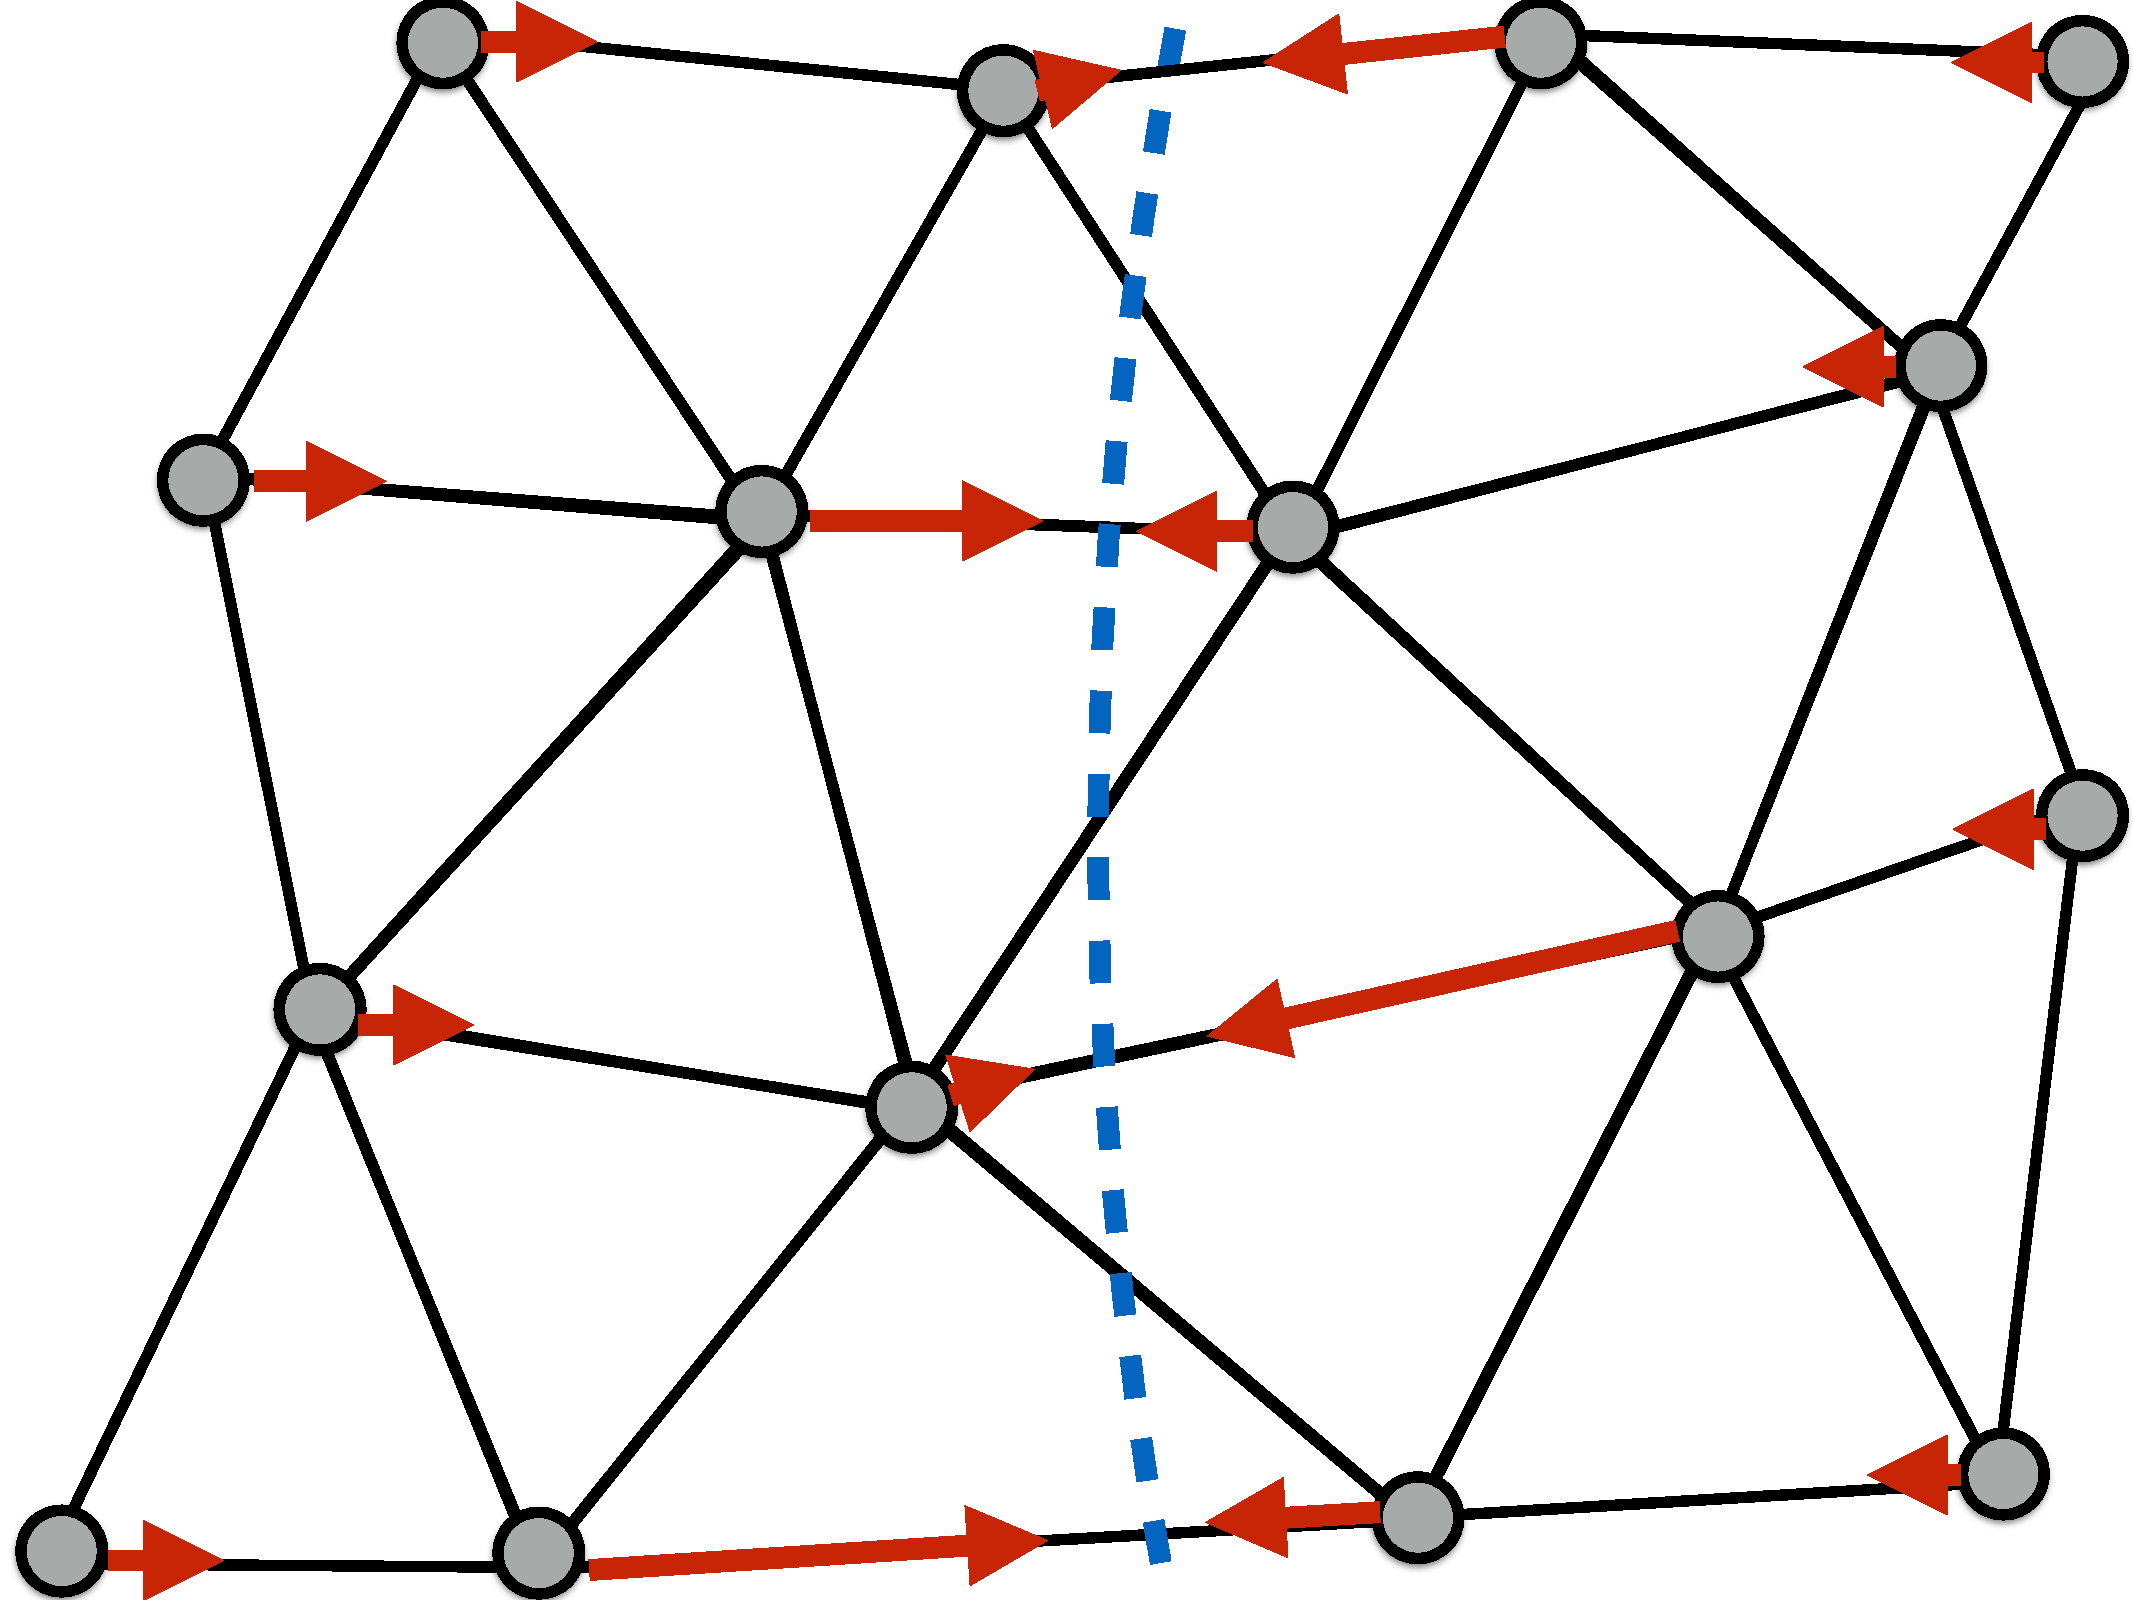
\includegraphics[width=0.47\textwidth]{figures/original-mesh-vec.pdf}
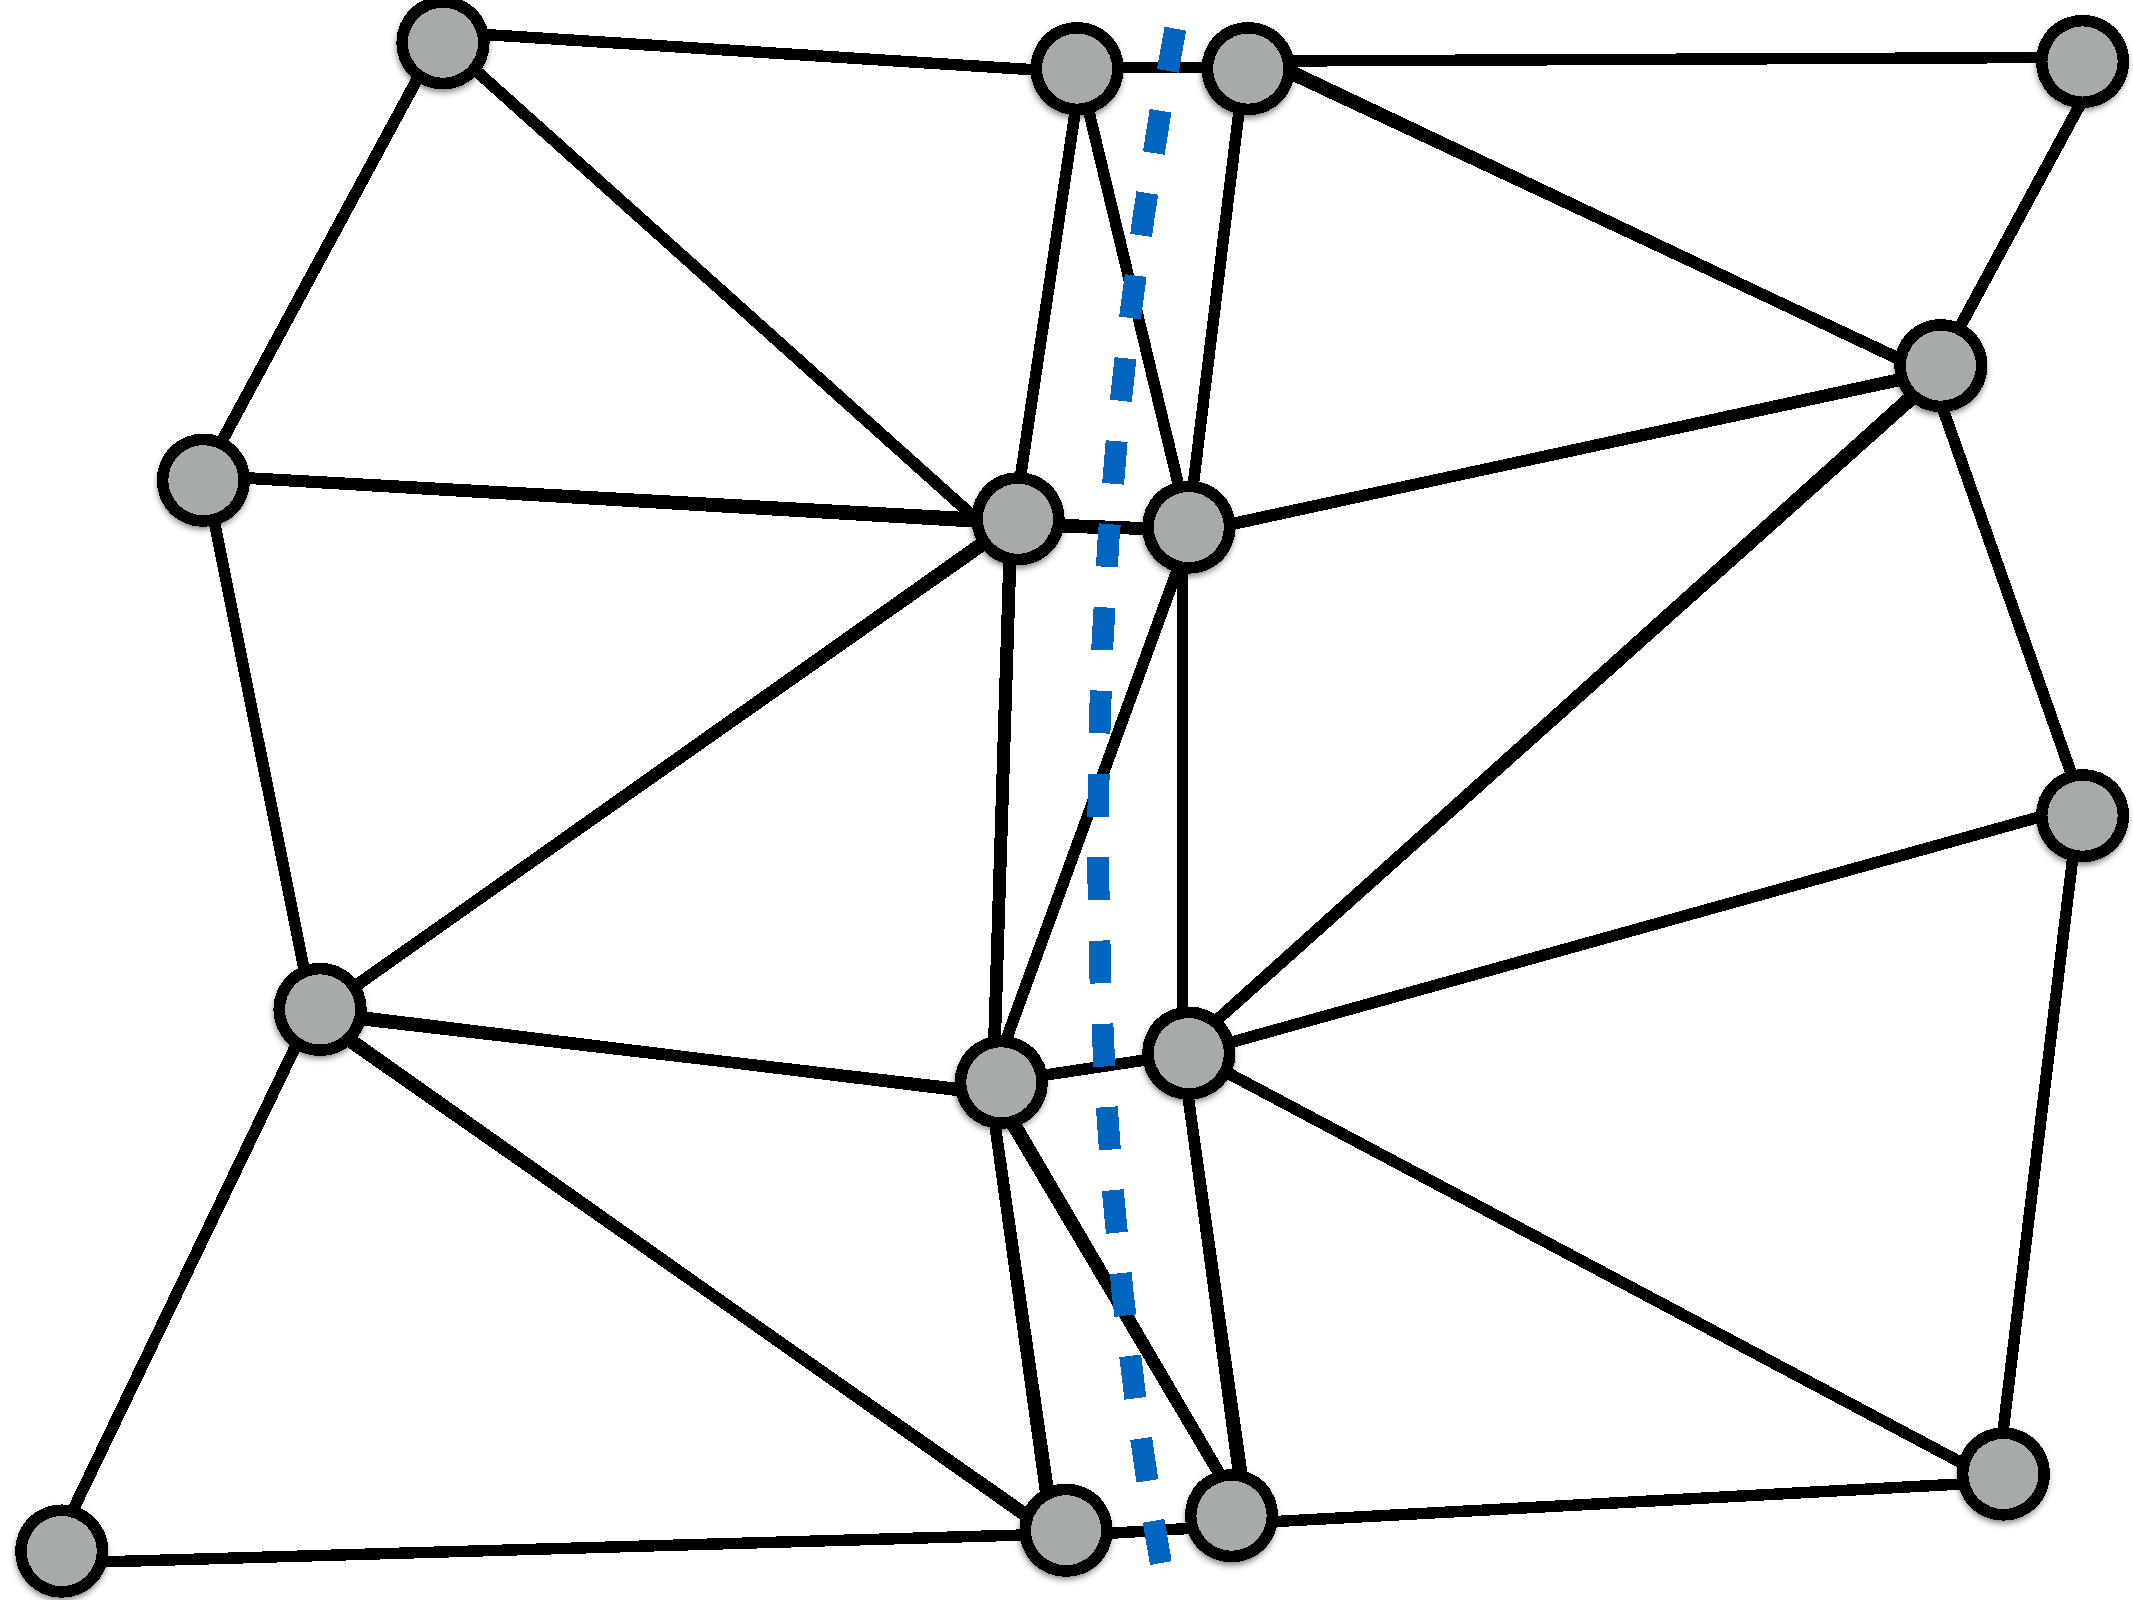
\includegraphics[width=0.47\textwidth]{figures/r-mesh2.pdf}
\caption{A sketched example of $r$-adaptation for shock waves where the original mesh with the desired displacement field ${\bf q}$ (arrows) is given on the left and the $r$-adapted mesh on the right. The shock wave is represented by the dashed line.}
\label{fig:moveboundary}\label{fig:sketch}
\end{center}
\end{figure} 
In the remainder of this section, we define the thermo-elastic formulation and the formulation of the thermal stresses that drive the $r$-adaptation strategy. 
\subsection{Thermal-elastic formulation}
Based on figure \ref{fig:sketch}, we are seeking a displacement vector field ${\bf q}_i=[q_{i,1},...,,q_{i,N}]^t$
 of each point in the domain $\Omega \in {R}^N$ where $N$ indicates
  the spatial dimension and where $q_i$ is the displacement in $i^{th}$ direction. 
  The linear thermo-elastic equations are given by
\begin{equation}\label{eq:linelas}
\nabla\cdot\left({\bf S}_e + {\bf S}_t\right) + {\bf f} = 0\hspace{10 mm}\in \Omega
\end{equation}
where ${\bf f}$ represents an arbitrary force in the 
domain and ${\bf S}_e$ is the stress tensor that is given by
\begin{equation}
{\bf S}_e = \lambda Tr({\bf E}){\bf I}+\mu {\bf E}
\end{equation}
${\bf I}$ denotes the identity matrix and the strain tensor ${\bf E}$ 
depends on the displacement vector ${\bf q}$ in the following way
\begin{equation}
{\bf E} = \frac{1}{2}\left(\nabla {\bf q}+(\nabla {\bf q})^t\right)
\end{equation}
The Lam\'e constants $\lambda$ and $\mu$ are described by the Young's modulus $\tilde{E}$ and the Poisson ratio $\nu$ and are written as
\begin{equation}
\lambda = \frac{\nu \tilde{E}}{\left(1+\nu\right)\left(1-2\nu\right)},\hspace{20 mm}\mu = \frac{\tilde{E}}{2\left(1+\nu\right)}
\end{equation}
In equation (\ref{eq:linelas}), the pseudo-thermal stress tensor is defined by ${\bf S}_t$.
Hence, we incorporate the concept of thermal expansion and contraction that
 is known from the theory of solid mechanics and use this as a mesh quality control mechanism.
For mesh quality control, the pseudo-thermal stress tensor ${\bf S}_t$ can depend on a quantity that indicates
 the level of deformity for each element. 
 Note that in the remainder of this article, the application of the thermal
  stress tensor in certain parts of the domain is often referred to
   as {\it heating} or {\it cooling down} the elements.

\subsection{Formulation of the thermal stress term}
The idea is to apply pseudo-thermal stresses to contract the elements in the vicinity of a shock wave. 
The discontinuity sensor presented in equation \ref{eq:sensor} is used to derive the pseudo-thermal stress terms. The value of $s_e$ is piecewise constant over the complete computational domain.
Hence, to take the divergence directly from the $s_e$ to formulate the pseudo-thermal stresses is undesirable because this leads zero gradients within each element and infinite gradients at the interfaces between elements. 
Therefore, we seek a smooth temperature distribution.
We use a similar analogy as the artificial diffusion model introduced by \cite{Barter2009} to compute a smooth distribution for $T_p$.
The following partial differential equation prescribes the diffusion of $s_e$ and is solved along with the governing equations in order to obtain a smooth pseudo-temperature distribution.
\begin{eqnarray}\label{eq:smoothvisc}
\frac{\partial {T_p}}{\partial t} = \sum_{i=1}^2 \frac{\partial^2 T_p}{\partial x_i^2} + \mu_a(s_e) -{T_p}; \qquad {{T_p}}\in \Omega
\end{eqnarray}
Generally, we consider a zero normal gradient for the pseudo-temperature on each type of boundary. Hence,
\begin{equation}
\sum_{i=1}^2\frac{\partial T_p}{\partial x_i}n_i = 0; \qquad {{T_p}}\in \Gamma
\end{equation}
Equation (\ref{eq:smoothvisc}) is a simplified version of the smooth artificial viscosity model that was introduced by Barter and Darmofal \cite{Barter2009}. In the thermo-elastic formulation discussed in this chapter, we use the solution that follows from equation (\ref{eq:smoothvisc}) 
\par One of the drawbacks of the model introduced in equation (\ref{eq:smoothvisc}) is that it makes the problem significantly more stiff. 
Hence, to calculate the smooth pseudo-temperature distribution, we first calculate the steady-state solution to the governing equations using the piecewise constant sensor distribution which is required anyway to compute the artificial diffusion term.
Once a steady-state is obtained, the computation is restarted and we use equation (\ref{eq:smoothvisc}) to determine the smooth temperature field. 
This is computationally cheaper than running the simulation with the additional equation for $T_p$ from the start.
The displacement of the nodes is then calculated based on the smooth pseudo-temperature.

\subsection{High-order spectral element continuous Galerkin (CG) discretisation}   

\section{Sensor-based $p$-adaptation}
\par We propose to use the discontinuity sensor given in equation (\ref{eq:sensor}) as an error indicator. A converged solution is calculated and based on the determined sensor value we define a set of threshold values. 
Based on a set  pre-defined sensor threshold values, we identify which elements required an increase in $p$.
For a range of $p_e \leq p \leq p_e+3$ for example, where $p_e$ represents the initial polynomial order which is typically low $(p_e = 2)$, we need three different threshold values namely, $s_1$, $s_2$ and $s_3$. 
\begin{equation*}\label{eq:switch}
   p^{\text{new}}_e
=\left \{ \begin{array}{l}
    p_e+3\hspace{20mm} \mbox{if}\hspace{20mm} s_e>s_{1}\\  
    p_e+2\hspace{20mm} \mbox{if}\hspace{20mm} s_{2}<s_e\leq s_{1}\\
    p_e+1\hspace{20mm} \mbox{if}\hspace{20mm} s_{3}<s_e\leq s_{2}\\
    p_e\hspace{27mm} \mbox{if}\hspace{20mm} s_e\leq s_{3}
    \end{array} 
    \right.
\end{equation*}
The number of required sensor values is dependent on the range of polynomial orders that 
one wants to use. 
These threshold values are determined by 
looking at the steady state sensor distribution. 
Based on these threshold values, 
a new polynomial distribution is obtained and this procedure is performed iteratively.
The expression given in equation \ref{eq:switch} is just an example.
The sensor value is typically high when a shock is detected. 
Hence, it is preferred to keep $p$ relatively low near at the shock wave to prevent numerical oscillations.
It is relatively straightforward to incorporate the capability to keep the polynomial order low above a certain value. 
The same variable $p$ implementation is used as the one described in \cite{Ekelschot2016}.
\section{Combining $r$- and $p$-adaptation}

\section{Numerical examples}

\subsection{Supersonic inviscid flow ($Ma=3.0$) past a forward facing step}
To illustrate the $r$-adaptation procedure, we compute inviscid supersonic flow $({Ma=3.0})$ 
past a forward facing step which has been thoroughly investigated by Woodward and Colella \cite{Woodward1984}. 
For this problem, we consider the compressible Euler equations and we neglect the effects of viscosity.
In the paper of Woodward and Colella \cite{Woodward1984}, the height of the step is taken to be $20\%$ of the height of the inlet so $h = 0.2H$ where in this case $H=2.0$. 
The conditions at the inlet were $\rho_\infty = 1.4$, $p_\infty=1$, $u_\infty=3.0$, $v_\infty = 0.0$. 
Woodward and Colella \cite{Woodward1984} presented results at $t=4.0$ since the steady-state solution does not show any interesting features other that the bow shock that is present upstream of the step.
These results presented at $t=4.0$ serve as reference data for current CFD code developers. However, in our case, we are interested is a configuration that results in shock reflections in the steady solution.
In this way we can study the suitability of $r$-adaptation when shock reflections and interactions occur. 
Therefore we have modified the height of the step from $h=0.2H$ to $h=0.175H$ as shown in \cite{Moura2016}. A detail of the initial mesh is shown in figure \ref{fig:dom_step}.
\begin{figure}[!htbp]
\begin{center}
\subfigure[The initial mesh.]
{
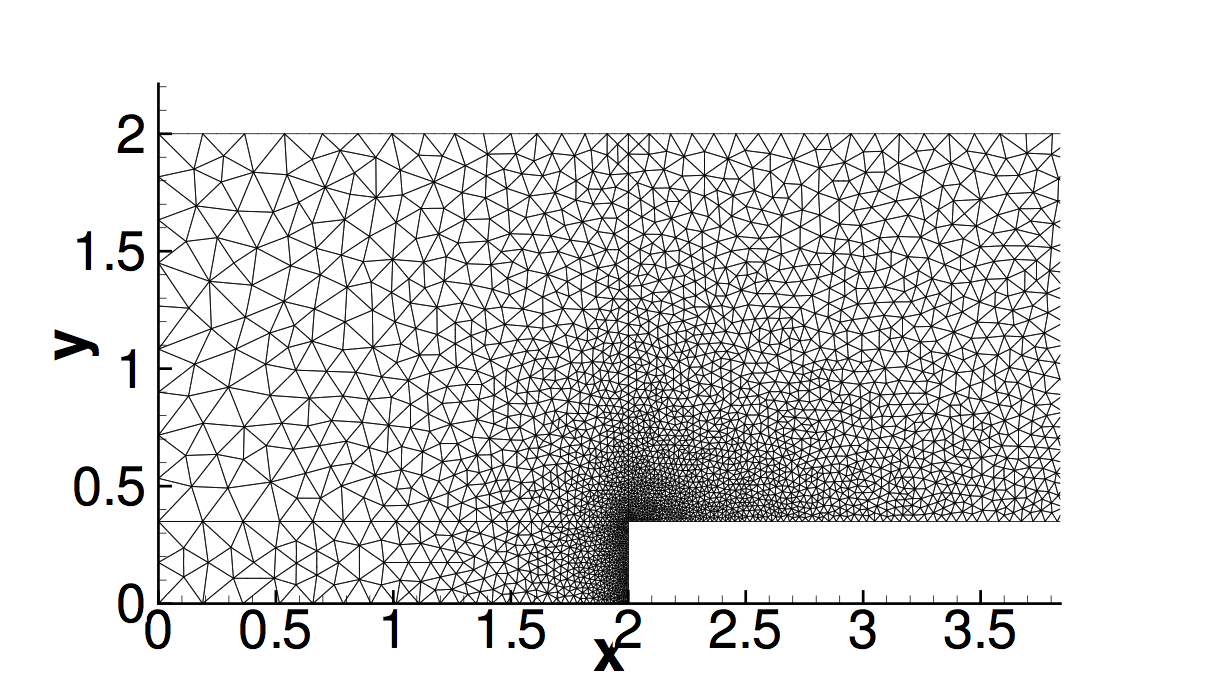
\includegraphics[width=0.47\textwidth]{figures/unref_mesh_nop.png}\label{fig:dom_step}
}
\subfigure[Mach number contours that are calculated using the initial mesh.]
{
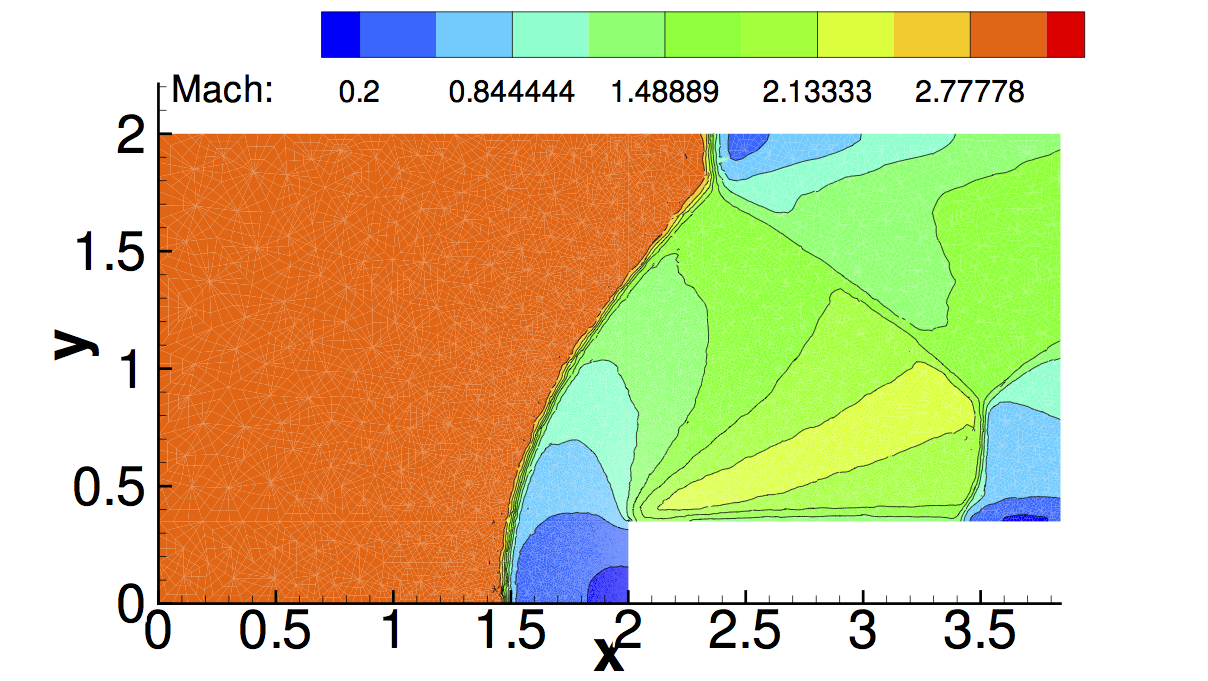
\includegraphics[width=0.47\textwidth]{figures/unref_mesh_Mach.png}\label{fig:step_MACH_P2}
}
\subfigure[Temperature distribution $T_p$ that is determined by solving equation (\ref{eq:smoothvisc}) along with the flow equations.]
{
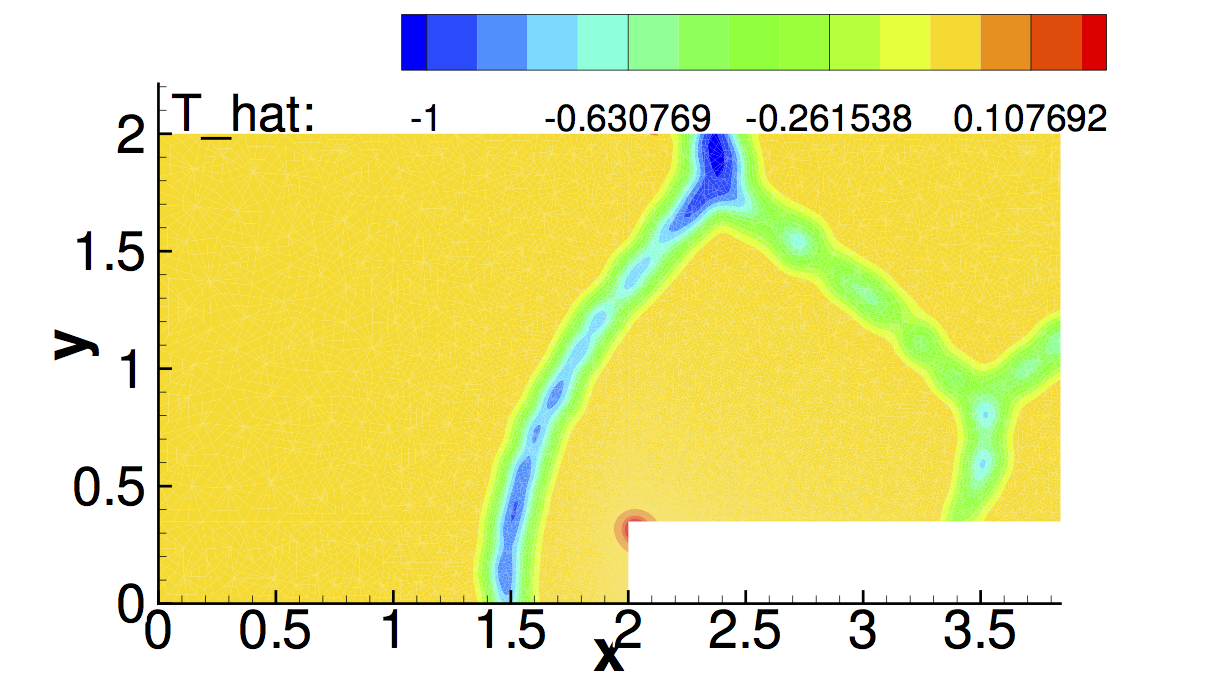
\includegraphics[width=0.47\textwidth]{figures/T_h_u.png}\label{fig:step_TEMP_P2}
}
\subfigure[The solution for $d_1$ of the thermo-elastic equations (first iteration) 
where the stream lines indicate how the degrees of freedom will move.]
{
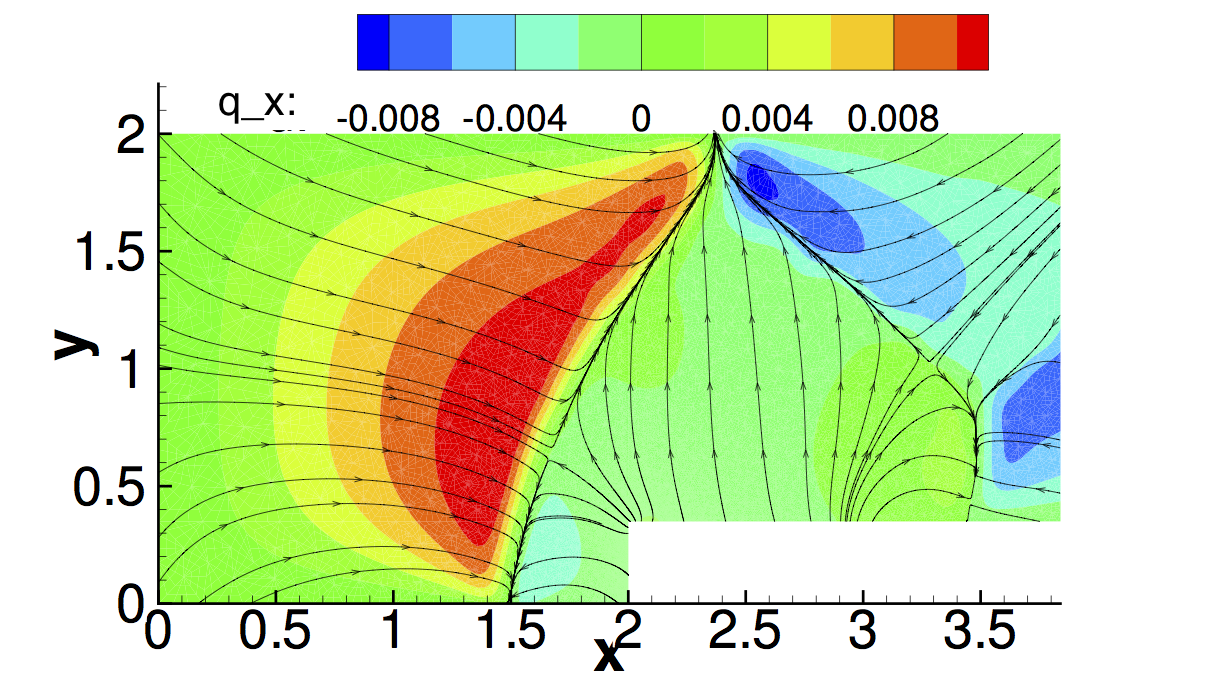
\includegraphics[width=0.47\textwidth]{figures/elas_u_retouch.png}\label{fig:xdisp}
}
\subfigure[Final $r$-adapted mesh after three iterations. ]
{
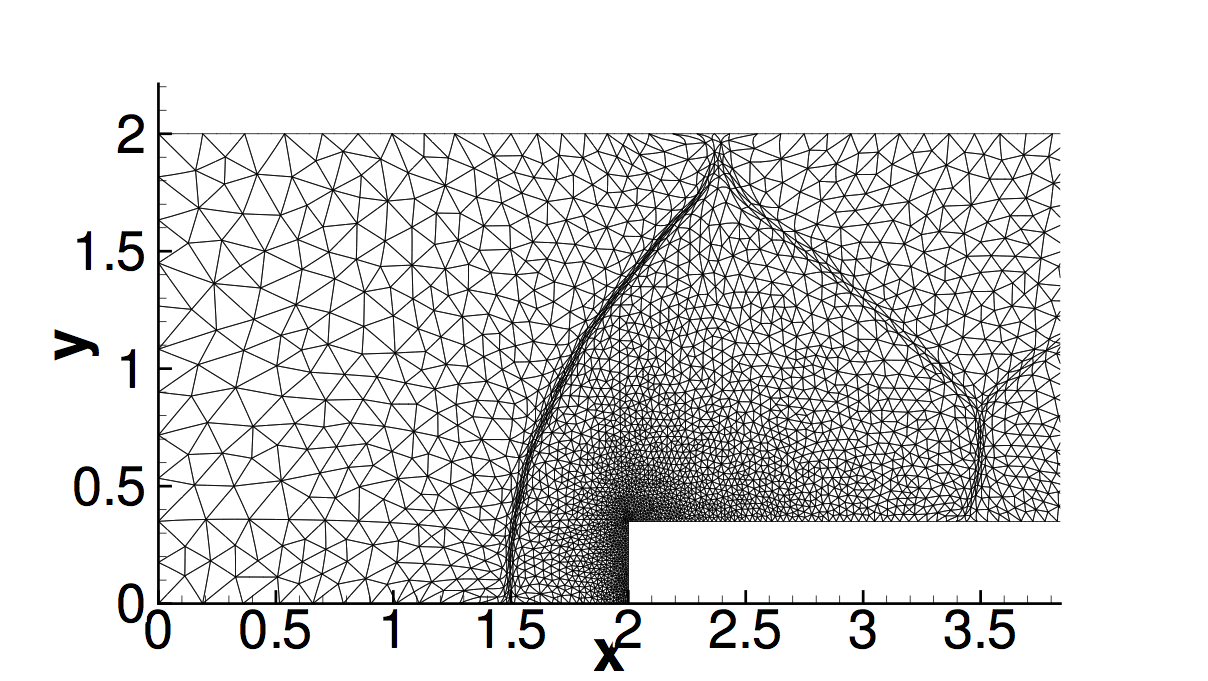
\includegraphics[width=0.47\textwidth]{figures/ref_mesh_nop.png}\label{fig:refmesh}
}
\subfigure[Mach number contours that are calculated after $r$-adaptation is applied.]
{
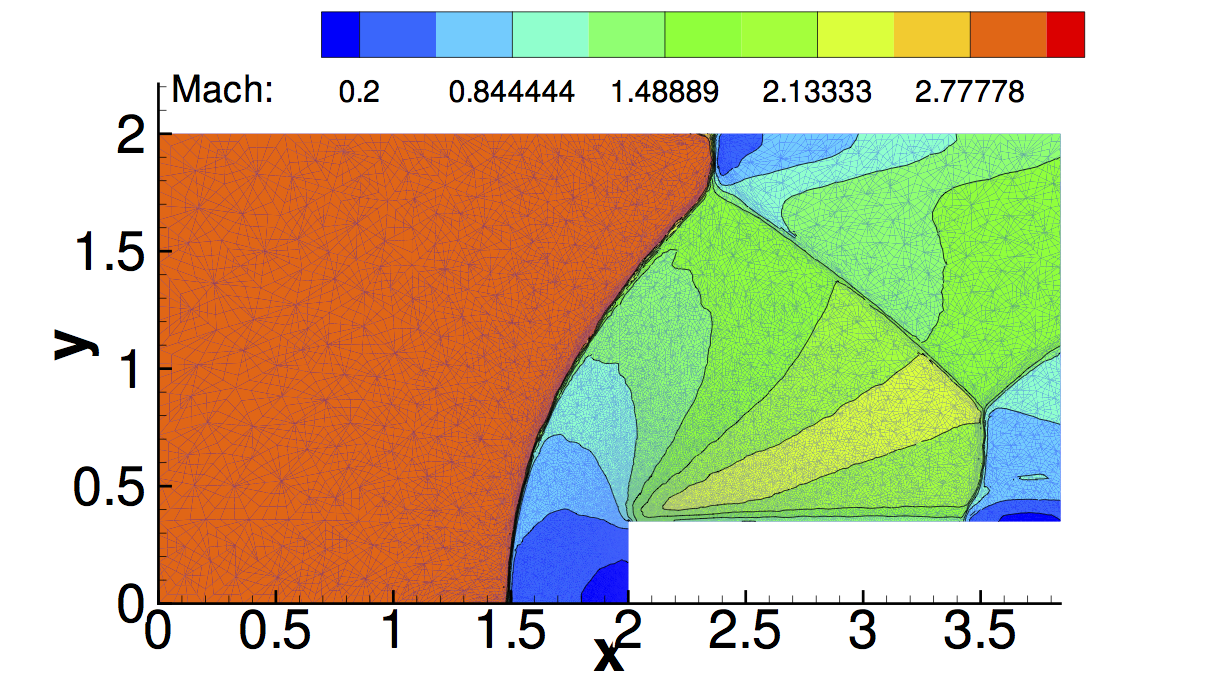
\includegraphics[width=0.47\textwidth]{figures/ref_mesh_Mach.png}\label{fig:refsteady}
}
\caption{General overview of the required steps to perform $r$-adaptation for supersonic inviscid flow past a forward facing step ($Ma=3.0$).}
\label{fig:radaptsteps}
\end{center}
\end{figure}
Figure \ref{fig:radaptsteps} illustrates the three main steps of the $r$-adaptation procedure.
We first obtain a low-order steady-state solution at $P=2$, shown in figure \ref{fig:step_MACH_P2}.
This figure shows that there is a strong bow shock downstream of the step. 
Furthermore, a strong normal shock forms at the upper wall where the bow shock reflects back. 
At the corner of the forward facing step, an expansion wave interacts with the 
reflected shock wave forming another normal shock at the lower wall.
We will use $r$-adaptation to accurately capture these flow features.
\par We use the discontinuity sensor to determine a smooth pseudo-temperature distribution which is shown in figure \ref{fig:step_TEMP_P2}.
Figure \ref{fig:step_TEMP_P2} shows that there is a significant variation in temperature because the bow shock and the normal shock at the upper wall are relatively strong compared to the weak reflection shock.
Based on the pseudo-temperature distribution, we obtain a displacement field of the nodes by solving the previously introduced thermo-elastic problem.
An example of the horizontal displacement component, $d_x$ is shown in figure \ref{fig:xdisp}. 
The streamlines indicate the direction in which the degrees of freedom are moving. 
Figure \ref{fig:xdisp} illustrates that the displacement field seems to be balanced at the top and elements are attracted from both sides to refine the normal shock at the upper wall.
\par Figures \ref{fig:refmesh} shows the resulting mesh after $r$-adaptation is applied. 
Furthermore, figure \ref{fig:refsteady} depicts the steady-state Mach contours that are obtained using the new mesh. 
Comparing figures \ref{fig:step_MACH_P2} and \ref{fig:refsteady} indicates that the representation of the bow shock and the reflecting shock waves further downstream is improved.
\par It has been noticed that the geometry of the step and the shock pattern further downstream have a significant influence of how well the $r$-adaptation procedure follows the curvature of the bow shock upstream of the step.
This is why two additional iterations were required to obtain the final mesh that was shown in figure \ref{fig:refmesh}
Initially, a pseudo-temperature field is calculated based on the sensor distribution obtained using the initial coarse mesh.
Based on this pseudo-temperature field, we calculate the deformation field.
The initial pseudo-temperature field together with the corresponding $d_x$ contours are given in figures \ref{fig:step_TEMP_P2} and \ref{fig:xdisp}.
From figure \ref{fig:xdisp} can be seen that there is a strong forcing in positive $x$-direction. However the forcing in opposite direction downstream of the bow shock is not as strong.
This causes an inaccurate overlap of the refinement and the location of the shock.
This is why two additional $r$-adaptation iterations were performed to ensure that the refinement corresponds well with the location of the shock.
%Figure \ref{fig:t1} depicts a more narrow pseudo-temperature distribution in the vicinity of the shock meaning that the location of the shock is determined more accurately.
%Figure \ref{fig:t2} eventually shows that the larger elements just upstream of the shock are 'cooled down' and contracted. However, in the upper part of the bow shock, as for the weaker shock just downstream of the bow shock, it is shown that the pseudo-temperature approaches zero and no extra refinement is required.
%Figure \ref{fig:dx2} illustrates that the forcing aligns the refinement with the physical location of the bow shock. 
\par To get more insight on this improvement, we compare the Mach distributions along three different $y$ positions, $y=0.5$, $y=0.75$ and $y=1.0$ which are shown in figure \ref{fig:line_plot_r_step}.
\begin{figure}[!htbp]
\begin{center}
\subfigure[Comparison of the Mach number between the original and the $r$-adapted mesh near the bow shock.]
{
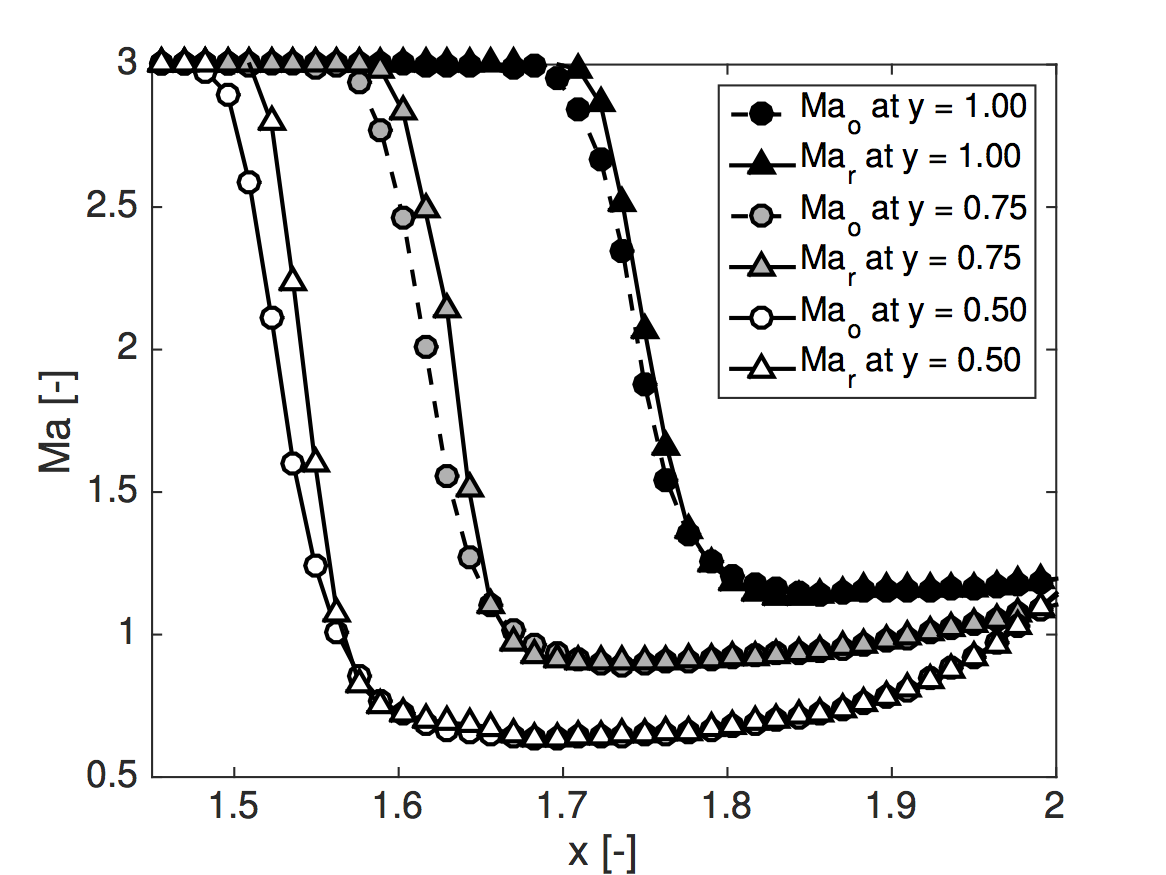
\includegraphics[width=0.47\textwidth]{figures/MACHDET1.png}\label{fig:lineplotFFS1}
}
\subfigure[Comparison of the Mach number between the original (circles) and the $r$-adapted (triangles) mesh near the normal shock.]
{
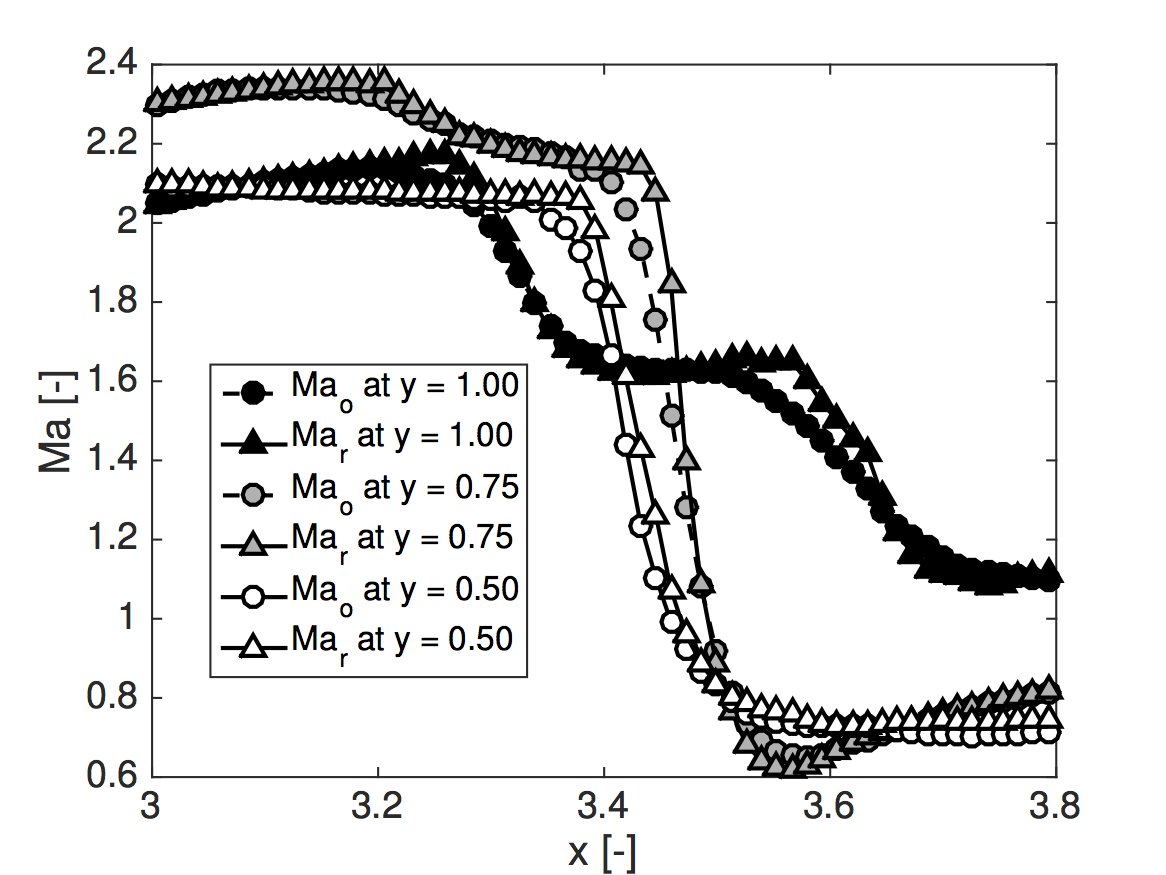
\includegraphics[width=0.47\textwidth]{figures/MACHDET2.png}\label{fig:lineplotFSS2}
}
\subfigure[Difference in Mach number between the original (circles) and the $r$-adapted (triangles) mesh near the bow shock.]
{
%\includegraphics[width=0.47\textwidth]{figures/DETAIL_MACH_ERROR.eps}\label{fig:diffLine1}
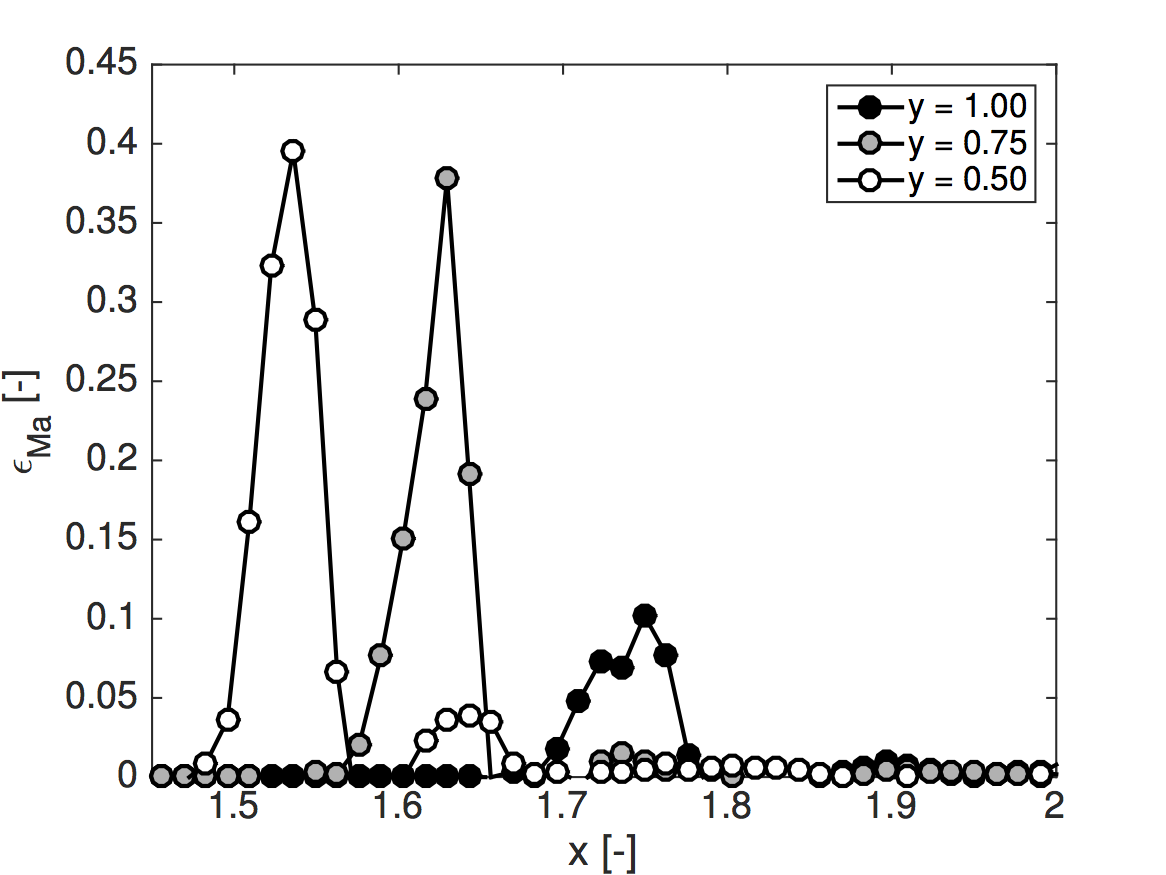
\includegraphics[width=0.47\textwidth]{figures/error_mach1.png}\label{fig:diffLine1}
}
\subfigure[Difference in Mach number between the original and the $r$-adapted mesh near the normal shock.]
{
%\includegraphics[width=0.47\textwidth]{figures/DMACH.eps}\label{fig:diffLine2}
\includegraphics[width=0.47\textwidth]{figures/error_mach2.png}\label{fig:diffLine2}
}
\caption{Comparison of the Mach number between the original and the $r$-adapted mesh at two locations: near the bow shock ($1.4\leq x \leq2$) and near the normal shock at the wall ($3\leq x \leq 3.8$).}
\label{fig:line_plot_r_step}
\end{center}
\end{figure}
In figures \ref{fig:lineplotFFS1} and \ref{fig:lineplotFSS2} the Mach number is plotted near the bow shock and near the normal shock on the lower wall downstream of the bow shock respectively. 
Figure \ref{fig:lineplotFFS1} shows the influence of the bow shock on each location.
Figure \ref{fig:lineplotFSS2} depicts the Mach number distribution further downstream of the bowshock at the normal shock. For $y=0.5$ and $y=0.75$ we see again a strong shock which corresponds to the normal shock located at $x\approx3.5$ while for $y=1.0$ shows two weak shocks which correspond with the shock reflections induced by the normal shock that occurs at approximately $(x,y) = (3.5,0.8)$. 
\par Figures \ref{fig:diffLine1} and \ref{fig:diffLine2} depict the error in Mach number  that is determined using
\begin{equation}
\epsilon_{Ma} =  \frac{\| Ma_o - Ma_r\|}{Ma_o}=\frac{\| \Delta Ma\|}{Ma_o}
\end{equation} 
where $Ma_o$ represent the Mach solution calculated using the original mesh and $Ma_r$ the Mach solution calculated using the final mesh after $r$-adaptation is applied.
At the bow shock $\Delta Ma = 0.48$ and $\Delta Ma = 0.6$ for $y=0.5$ and $y=0.75$ respectively while for $y=1.0$ we find that $\Delta Ma = 0.2$.
%The shock thickness generally depends on the difference between Mach number upstream and downstream of the shock.
Naturally, $\Delta Ma$ depends on the difference in Mach number upstream and downstream of the shock.
Hence, it is expected that a large $\Delta Ma$ is obtained for stronger shocks. 
Both figures \ref{fig:diffLine1} and \ref{fig:diffLine2} show that $\epsilon_{Ma}$ is largest when the difference between $v_1$ and $v_d$ is biggest as well. It is assumed that the discretisation is generally much coarser than the anticipated shock thickness. 
Hence, it is expected to have the biggest gain in accuracy when the difference between the Mach number upstream and downstream of the shock is larger.

\subsection{Transonic inviscid flow ($Ma=0.8$) past a NACA 0012 at an angle of incidence of $\alpha=1.25^\circ$}
We investigate the performance of $r$-adaptation strategy using the thermo-elastic analogy for the well-known test case of transonic inviscid flow ($M = 0.8$) past a NACA 0012 aerofoil at an angle of attack of $1.25^\circ$. 
The domain around the NACA $0012$ profile is discretised using an unstructured mesh of $6470$ triangular elements. 
This is the same test case as the one presented in section \ref{sec:DLRNEK}. Hence, we obtain a strong shock on the suction side at approximately $60\%$ of the chord and a weak shock on the pressure side at approximately $35\%$ of the chord. 
Initially, a flow solution is computed using a uniform polynomial order of $P=2$.
The original mesh and the flow solution obtained using $P=2$ is shown in figures \ref{fig:iniMesh} and \ref{fig:iniMach} respectively.
\begin{figure}[!htbp]
\begin{center}
\subfigure[Mach contours obtained using the initial mesh with a uniform $p=2$.]
{
%\includegraphics[width=0.47\textwidth]{figures/origin_sm_25.eps}\label{fig:iniMesh}
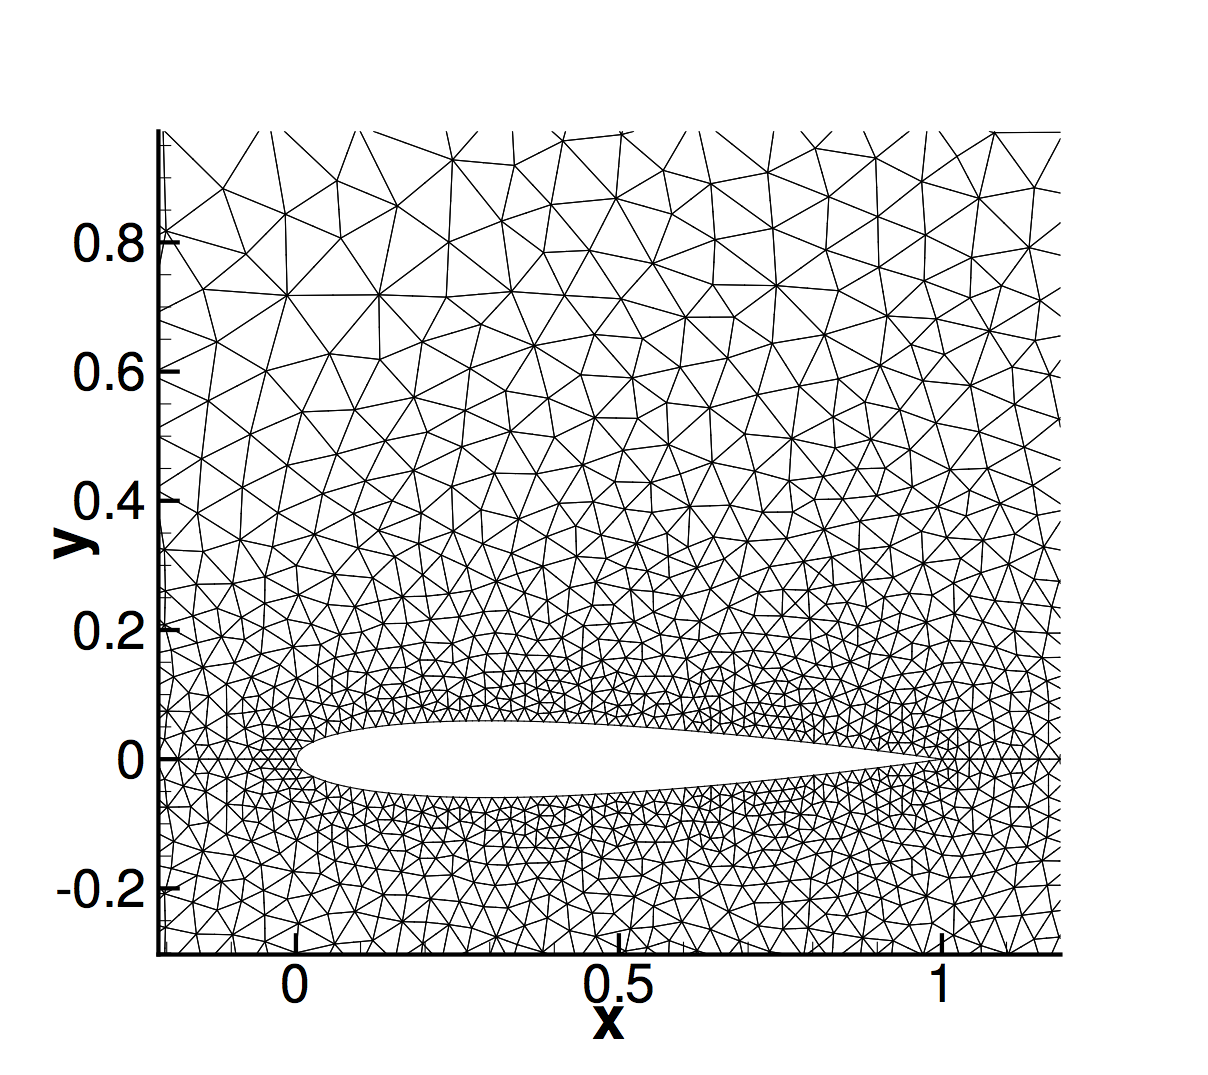
\includegraphics[width=0.47\textwidth]{figures/0-mesh.png}\label{fig:iniMesh}
}
\subfigure[Mach contours obtained using the initial mesh with a uniform $p=2$.]
{
%\includegraphics[width=0.47\textwidth]{figures/norefMach.png}\label{fig:iniMach}
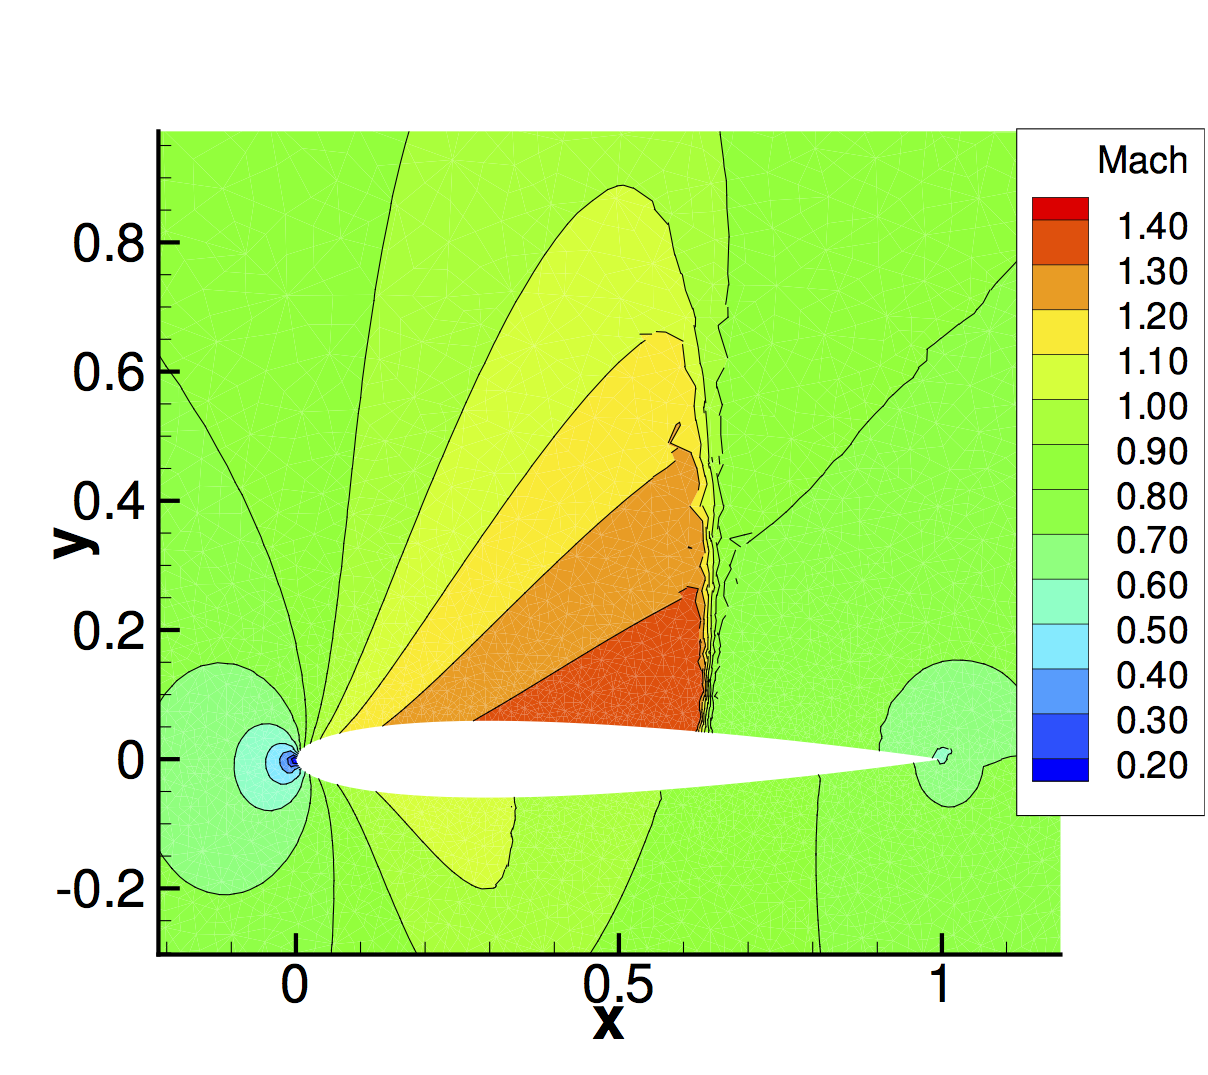
\includegraphics[width=0.47\textwidth]{figures/M0-trans2.png}\label{fig:iniMach}

}
\subfigure[$T_p$ contours based on the steady-state sensor solution.]
{
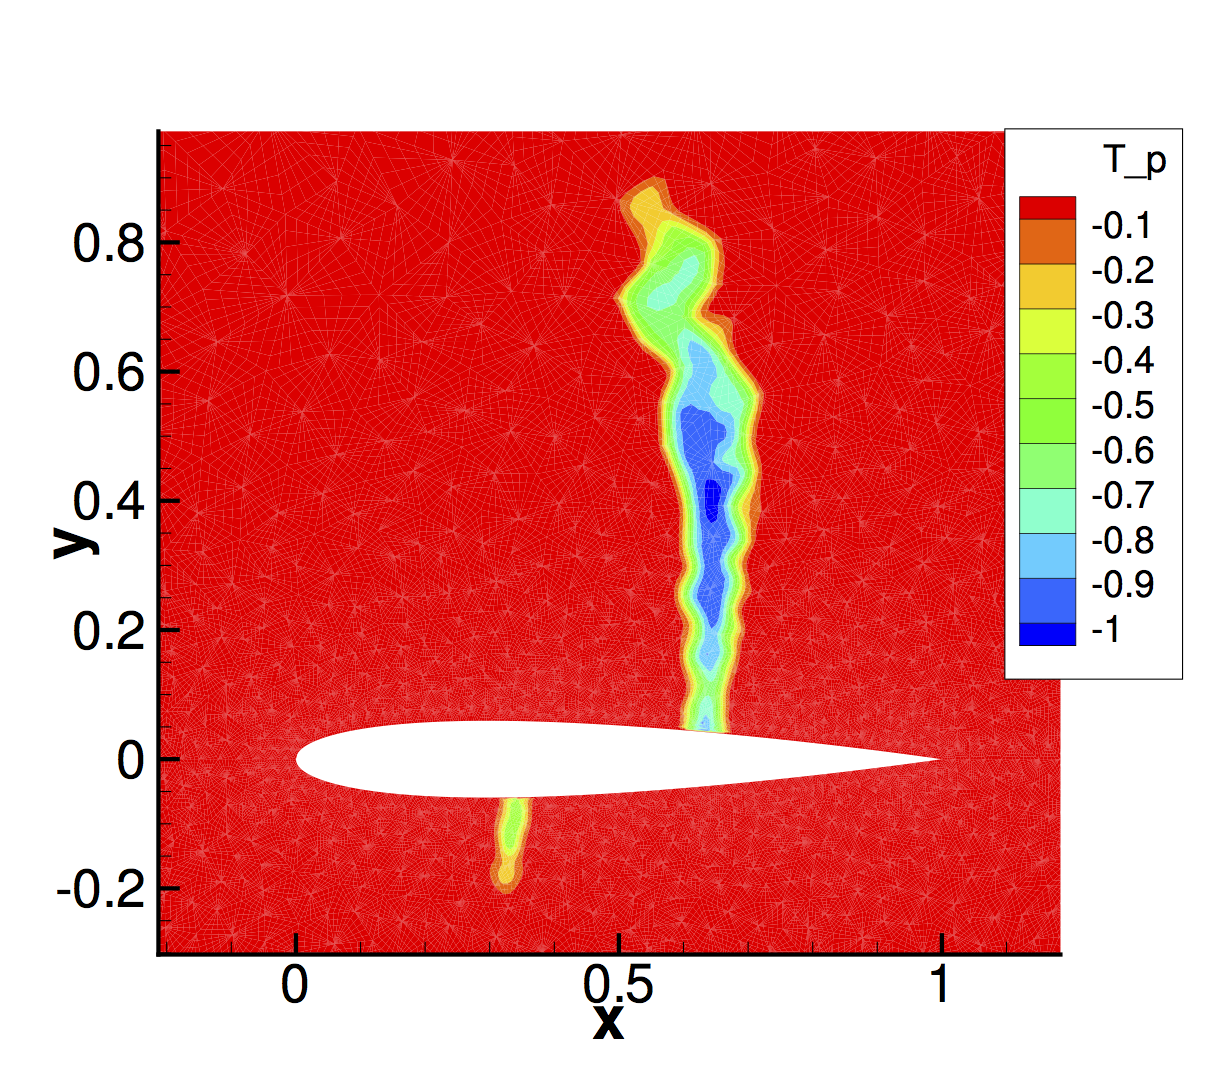
\includegraphics[width=0.47\textwidth]{figures/Tp-trans.png}\label{fig:temperature}
}
\subfigure[$d_x$ contours plotted with the streamlines that indicate how the nodes will move.]
{
%\includegraphics[width=0.47\textwidth]{figures/u_ini_v2.png}\label{fig:uini}
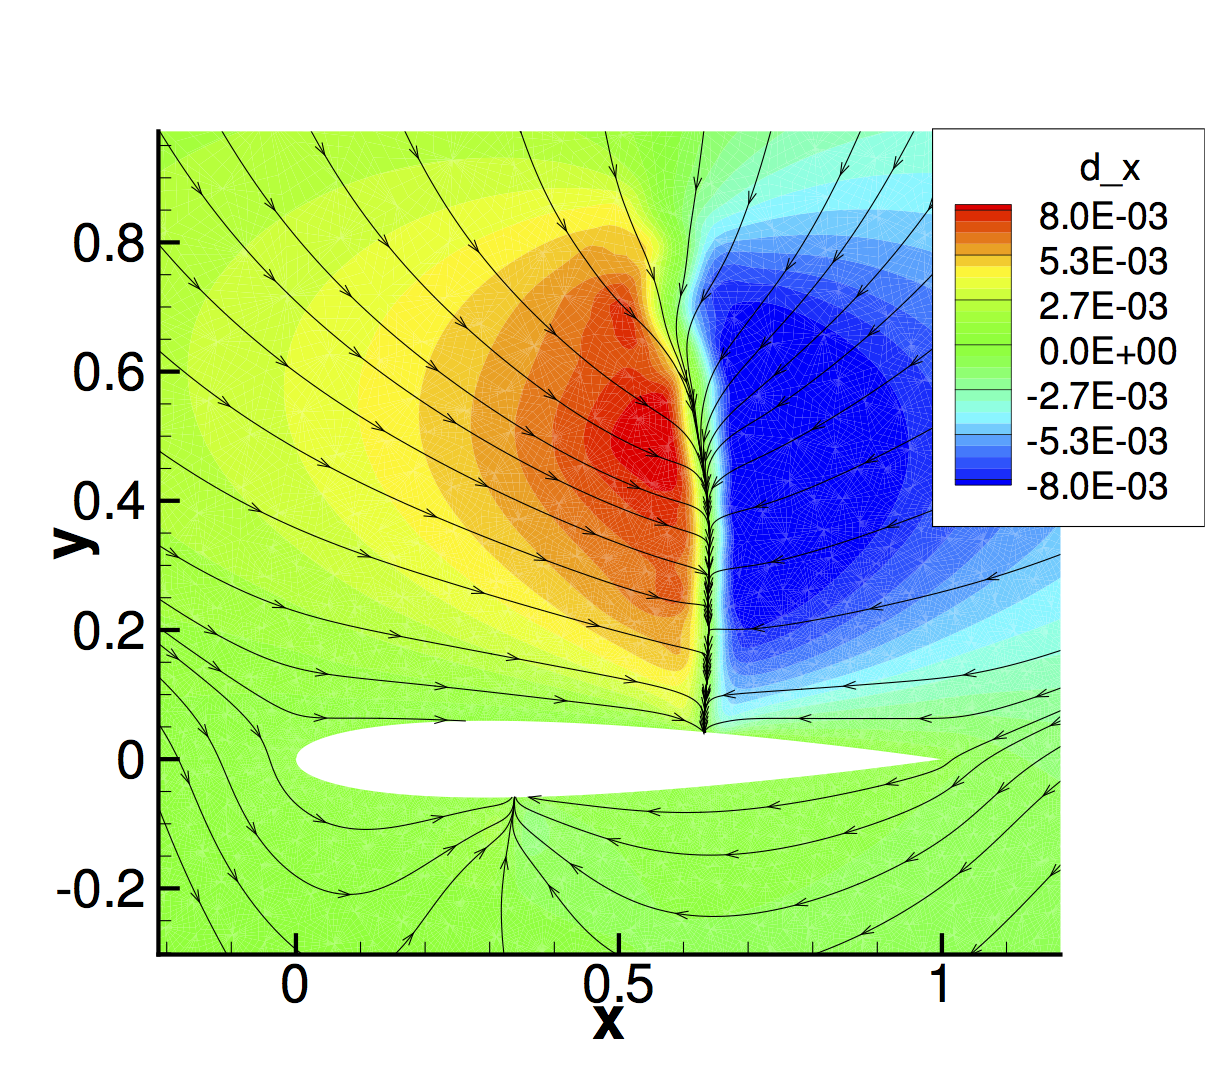
\includegraphics[width=0.47\textwidth]{figures/dx-trans.png}\label{fig:uini}
}
%\subfigure[The $q_x$ solution after $15$ iteration steps.]
%{
%\includegraphics[width=0.47\textwidth]{figures/u_15_v2.png}\label{fig:u15}
%}
%\subfigure[The $q_x$ solution after $30$ iteration steps.]
%{
%\includegraphics[width=0.47\textwidth]{figures/u_30_v2.png}\label{fig:u30}
%}
\subfigure[Mach contours obtained using the $r$-refined mesh with a uniform $p=2$.]
{
%\includegraphics[width=0.47\textwidth]{figures/mesh_sm_25.eps}\label{fig:finalMesh}
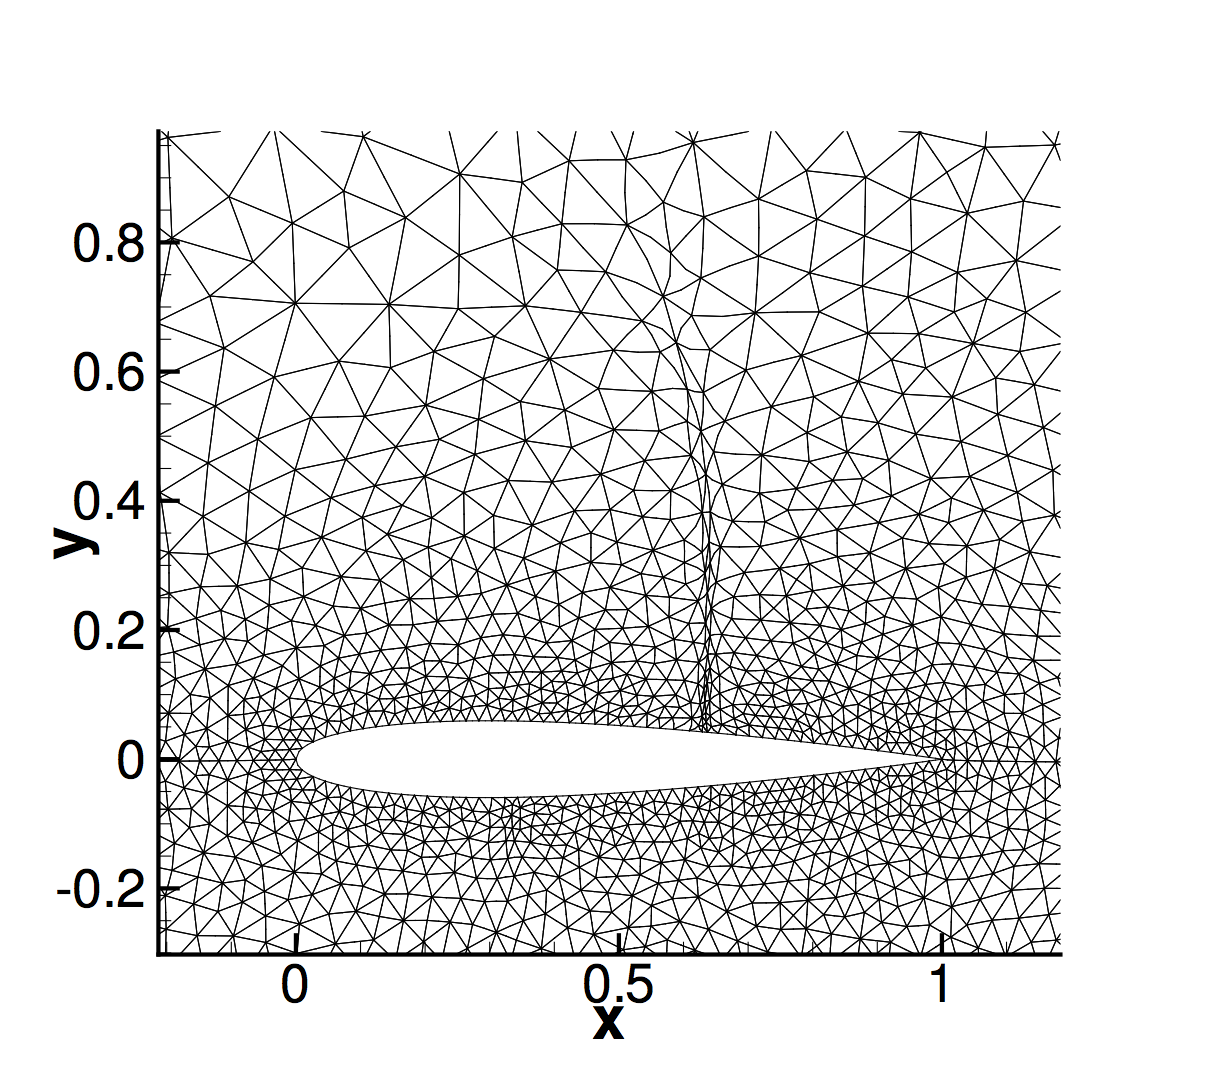
\includegraphics[width=0.47\textwidth]{figures/r-mesh.png}\label{fig:finalMesh}
}
\subfigure[Mach contours obtained using the $r$-refined mesh with a uniform $p=2$.]
{
%\includegraphics[width=0.47\textwidth]{figures/rrefMach.png}\label{fig:finalMach}
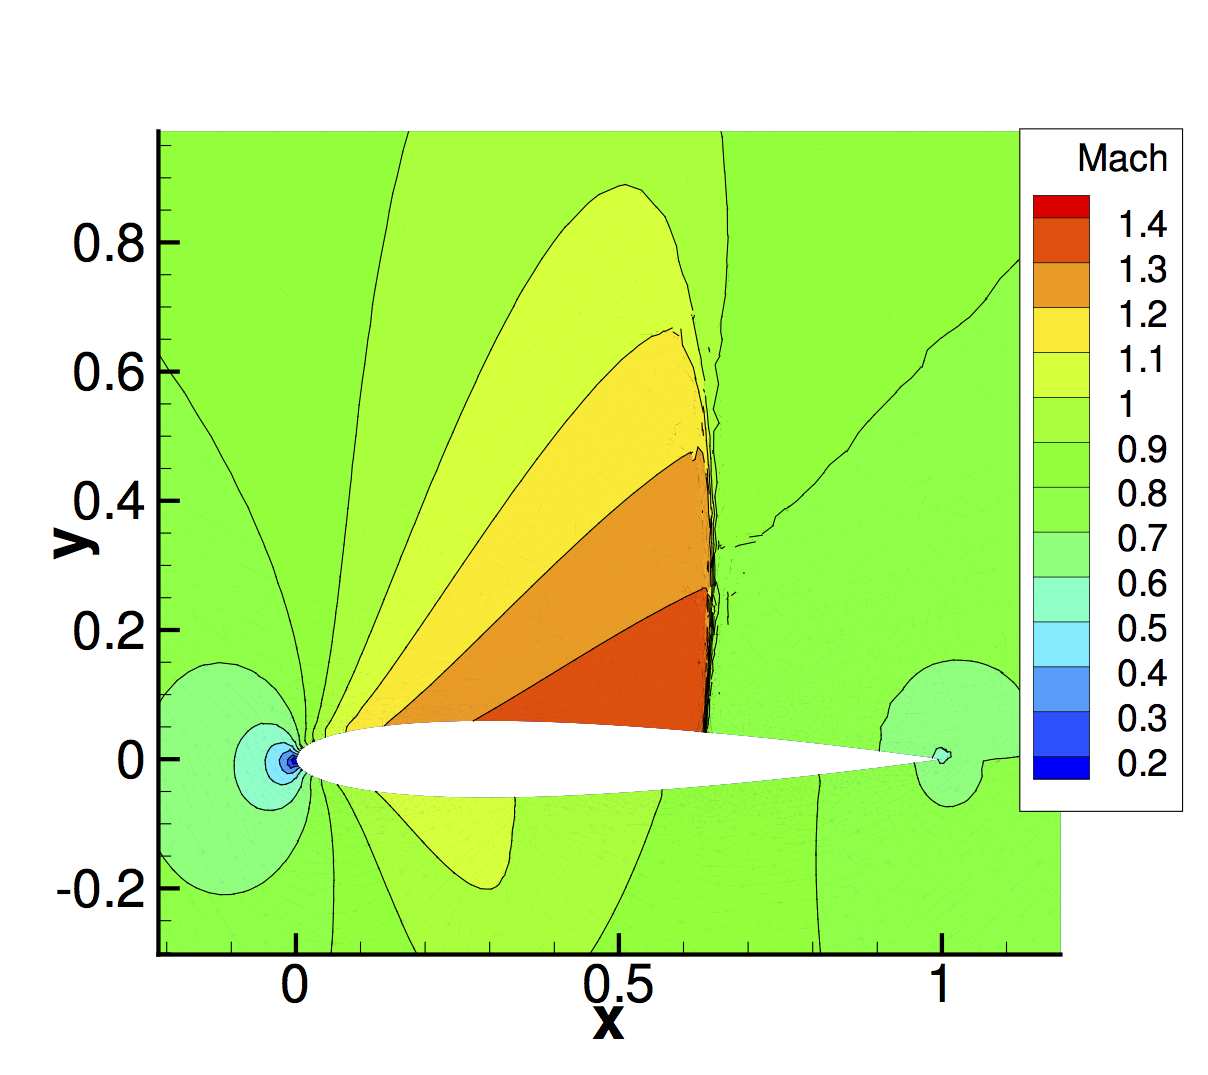
\includegraphics[width=0.47\textwidth]{figures/Mr-trans.png}\label{fig:finalMach}
}
\caption{Visualisation of the $r$-adaptation procedure for inviscid transonic flow past a NACA 0012 aerofoil (${Ma=0.8}$, $\alpha = 1.25^\circ$).}
\label{default}
\end{center}
\end{figure}



The smooth pseudo-temperature distribution is calculated using equation (\ref{eq:smoothvisc}) and is shown in figure \ref{fig:temperature}. 
This pseudo-temperature field is used to contract the elements that cover the shocks. 
Based on this pseudo-temperature, we calculate the displacement field of the degrees of freedom according to the thermo-elastic equations.
In figure \ref{fig:uini}, the streamlines are plotted which indicate how the nodes are going to move. 
This figure illustrates that the elements that cover the strong shock on the suction side and the elements that cover the weak shock on the pressure side are going to contract. 
After $r$-adaptation is applied we determine the final mesh which is shown in figure \ref{fig:finalMesh}. 
Finally, this mesh is used to calculate the refined flow solution which is illustrated in figure \ref{fig:finalMach}.
By comparing figure \ref{fig:iniMach} with \ref{fig:finalMach}, we conclude that particularly the representation of the strong shock on the suction side is significantly improved.
The $r$-adaptation procedure for this particular case takes about three to five minutes on four CPU's on a personal laptop. This is negligible compared to the time it takes to solve the governing equations.
\par For optimal performance of the $r$-adaptation strategy we need to allow the nodes to move freely along the wall boundary edge. 
Figure \ref{fig:mm} shows a detailed comparison of the original mesh and the $r$-adapted mesh at the root of the strong shock on the suction side.


\begin{figure}[!htbp]
\begin{center}
\subfigure[Detail of the comparison between the original mesh (thin grey lines) and the mesh after $r$-adaptation is applied (thick black lines) at the root of the strong shock at the suction side.]
{
%\includegraphics[width=0.47\textwidth]{figures/detail_wall3.eps}\label{fig:mm}
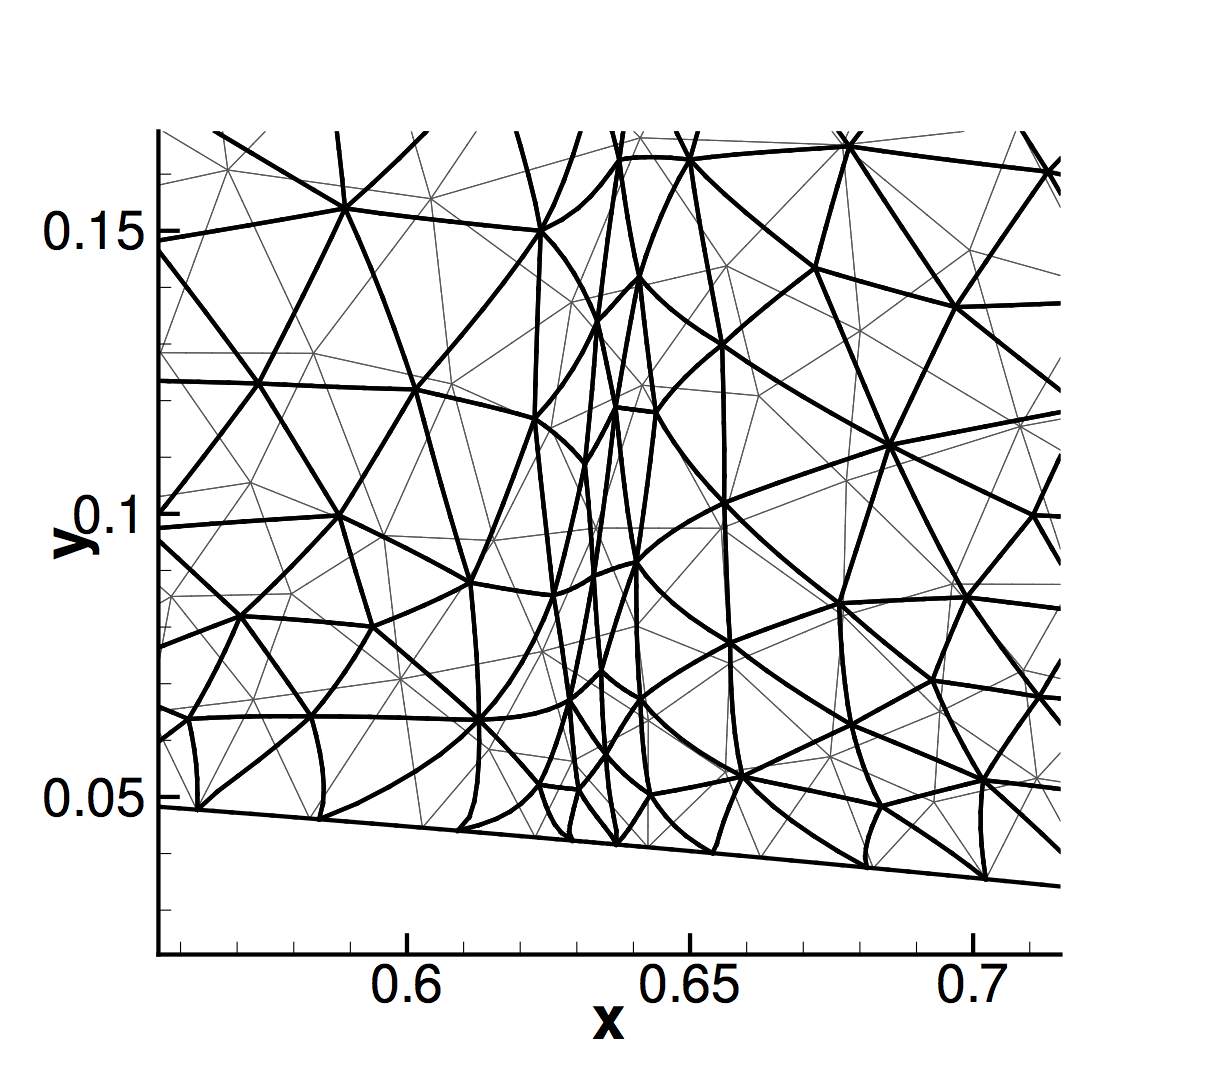
\includegraphics[width=0.47\textwidth]{figures/mesh_root.png}\label{fig:mm}
}
\subfigure[Detail of the comparison between the original mesh (thin grey lines) and the mesh after $r$-adaptation is applied (thick black lines) away from the geometry near the shock at the suction side.]
{
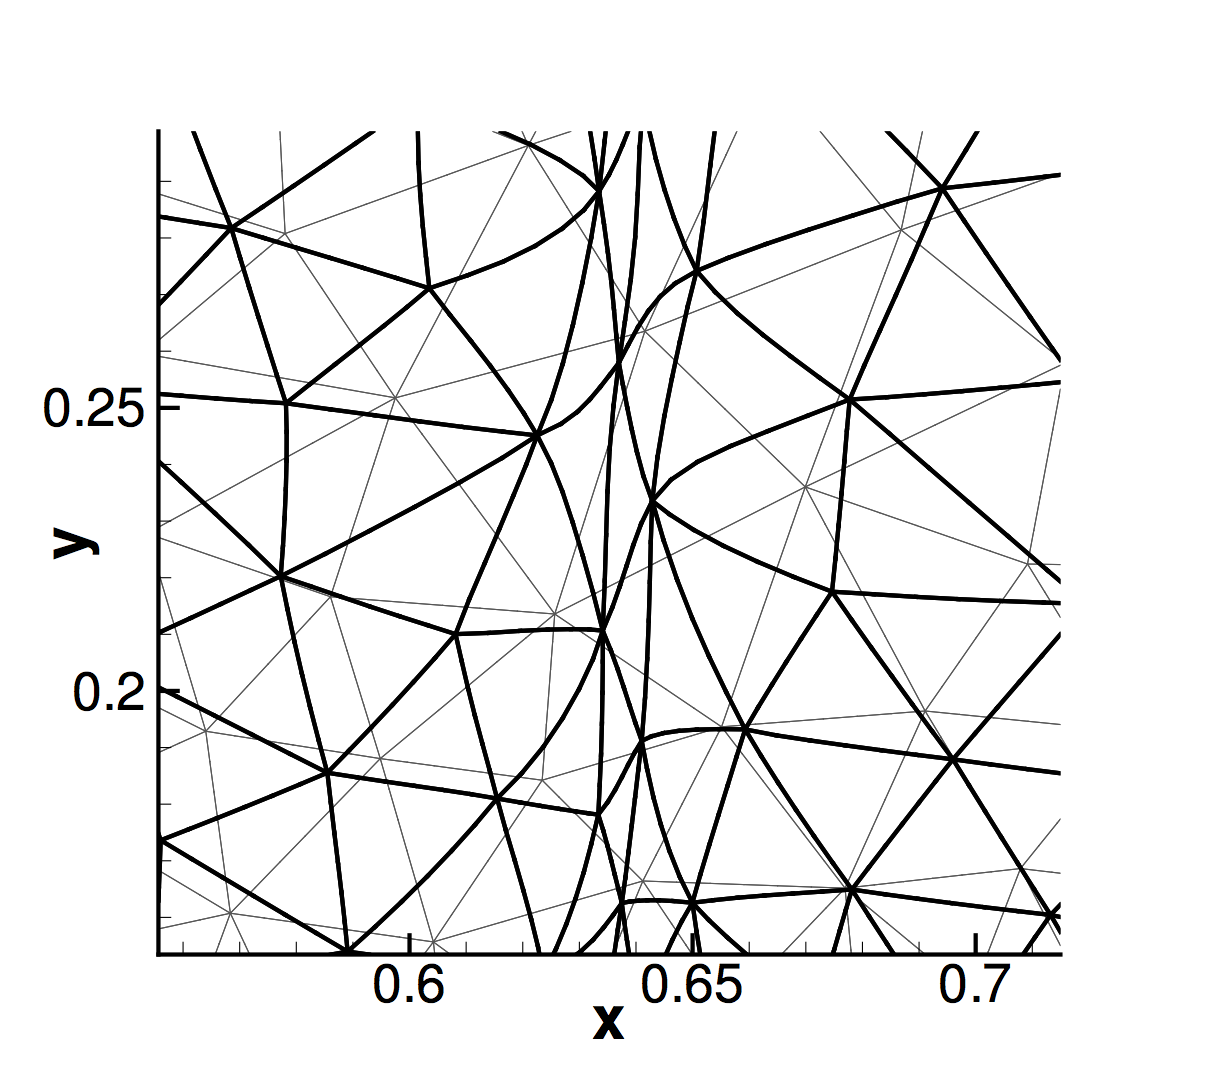
\includegraphics[width=0.47\textwidth]{figures/mesh_det.png}\label{fig:mm2}
}
\caption{Detailed comparison between the original mesh and the mesh after $r$-adaptation at the suction side of the NACA $0012$.}
\end{center}\label{fig:detailradapt}
\end{figure}


\begin{figure}[!htbp]
\begin{center}
\subfigure[Comparison of the Mach solution at wall obtained using the original and $r$-adapted mesh.]
{
%\includegraphics[width=0.47\textwidth]{figures/wall_overview.eps}\label{fig:walltrans}
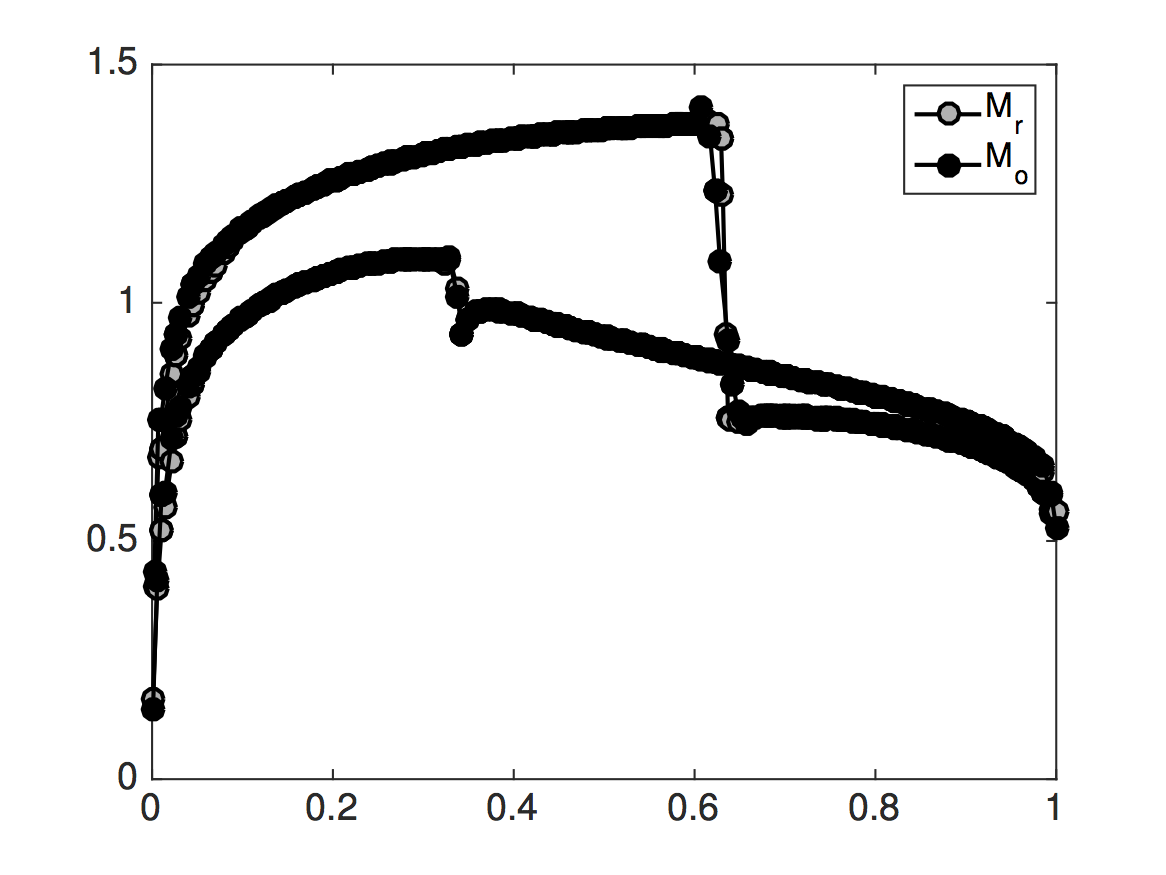
\includegraphics[width=0.47\textwidth]{figures/ww.png}\label{fig:walltrans}
}
\subfigure[Detailed comparison of the Mach solution at the root of the strong shock on the suction side obtained using the original and $r$-adapted mesh.]
{
%\includegraphics[width=0.47\textwidth]{figures/comp_wall_trans.eps}\label{fig:walltrans_det}
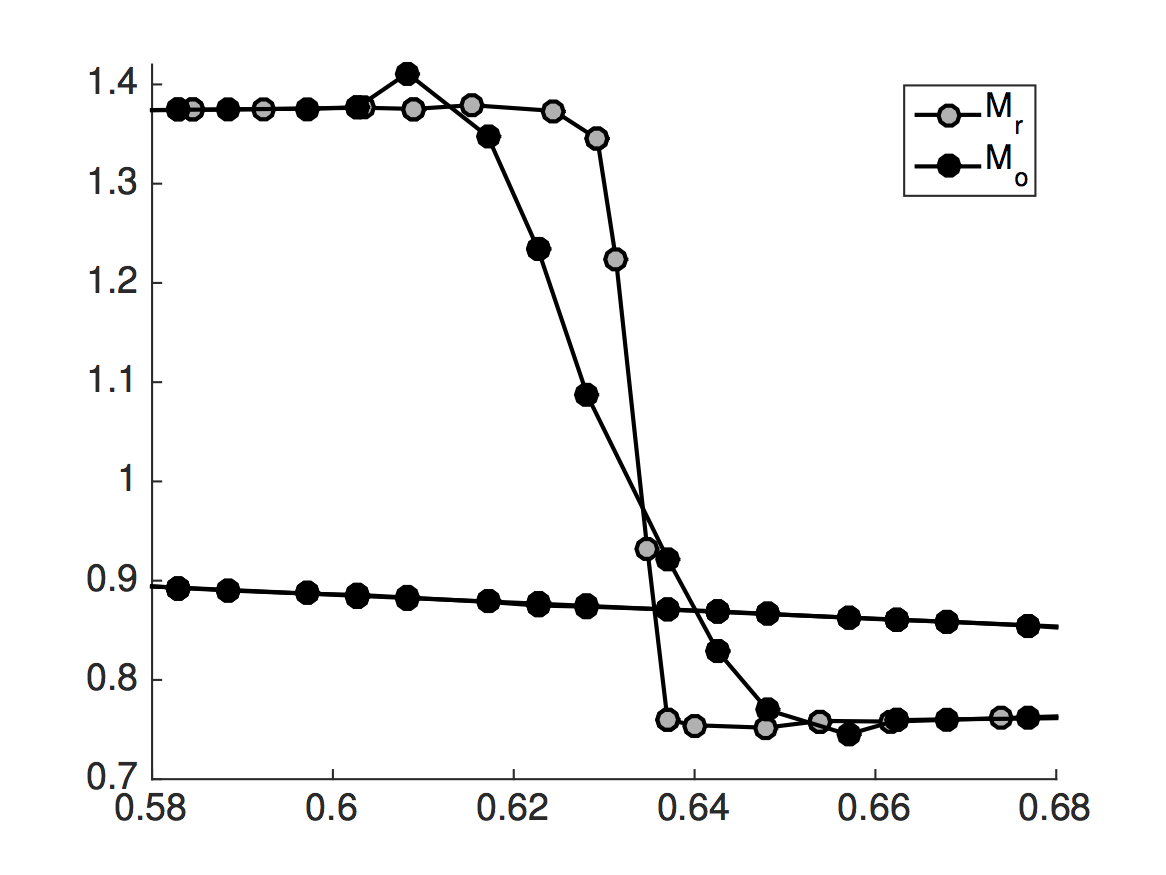
\includegraphics[width=0.47\textwidth]{figures/ww_det.png}\label{fig:walltrans_det}
}
\caption{Comparison between the Mach distribution obtained using the original mesh (black dots) and the mesh after $r$-adaptation is applied (grey dots).}
\label{fig:machtranswall}
\end{center}
\end{figure}
The detailed picture of the Mach solution at the strong shock on the suction side, given in figure \ref{fig:walltrans_det}, shows particularly well the improvement that is obtained using the $r$-adapted mesh.
Both cases use the same amount of artificial diffusion.
The solution for $Ma_0$ shows small wiggles both upstream and downstream of the shock which are completely removed for $Ma_r$.
Furthermore, as expected, a significantly stronger gradient at the shock is obtained using the $r$-adapted mesh.
This corresponds with the shock thickness estimation. 
\par The high curvature of the elements can cause aliasing since the Jacobian of the mapping in included as a polynomial function is the integral over the elemental area.
Hence, it was noticed that for the highly curved elements, for example at the top of the strong shock on the suction side, de-aliasing techniques should be applied to prevent numerical instabilities.
However it is also noticed that the elements are deformed in the direction of the shock wave.
Hence, the slide boundary conditions work well up to point that the surrounding elements become invalid.
This is prevented by implementing a combination of the previously introduced mesh validity control strategy using one of mesh quality indicators proposed section \ref{sec:meshqual}. 
The mesh quality control parameter is used to increase the local stiffness coefficient of the element preventing it to become invalid.
This also requires an appropriate stopping criteria which has not been incorporated in this study.
\section{Conclusions}
In this article, we proposed a $r$-adaptation capability that relies on a thermo-elastic formulation in order to improve the solution accuracy in the vicinity of shock waves while maintaining the same number of degrees of freedom. We have demonstrated the effectiveness of the proposed $r$-adaptation strategy using two test cases: The first test case considered was supersonic flow past a forward facing step and the second test case demonstrated the combination of $r$-adaptation with goal-oriented $p$-adaptation.
\par {\bf Describe conclusions based on test case 1}
\par {\bf Describe conclusions based on test case 2}
\par The proposed $r$-adaptation capability maintains the mesh connectivity so there is no need to repartition the mesh once the computation is restarted. In this article we have considered only steady flows.	However, this is potentially an attractive method for unsteady $r$-adaptation since there is no additional re-meshing or repartitioning step required.
\par Furthermore, it is recommended to incorporate the proposed $r$-adaptation strategy in a quad- or hex-dominant mesh environment since these types of meshes are very suitable to approximate large gradients like boundary layers and shock waves.
\section*{References}

\bibliography{rp-biblio}

\end{document}